% Approximate multiplication inside a DNN on a multiplierless RISC-V CPU, explained from scratch.
% Build:  cd doc && python3 make_figures.py && pdflatex roba_explained && pdflatex roba_explained
\documentclass[11pt,a4paper]{article}

\usepackage[T1]{fontenc}
\usepackage[utf8]{inputenc}
\usepackage{lmodern}
\usepackage{microtype}
\usepackage[margin=2.3cm]{geometry}
\usepackage{amsmath,amssymb}
\usepackage{graphicx}
\usepackage{booktabs,tabularx,multirow,makecell}
\usepackage{xcolor}
\usepackage{enumitem}
\usepackage{caption}
\usepackage{float}
\usepackage{listings}
\usepackage[most]{tcolorbox}
\usepackage{tikz}
\usetikzlibrary{positioning,arrows.meta,calc,fit,shapes.geometric,matrix,decorations.pathreplacing}
\usepackage[colorlinks=true,linkcolor=blue!50!black,urlcolor=blue!50!black,citecolor=blue!50!black]{hyperref}

\setlength{\parskip}{0.45em}
\setlength{\parindent}{0pt}
\setlength{\emergencystretch}{3em}
\setlist{itemsep=0.15em,topsep=0.3em}
\captionsetup{font=small,labelfont=bf}
\graphicspath{{figures/}}

% ---------------------------------------------------------------- colours used in every figure
\definecolor{exact}{HTML}{3B4351}
\definecolor{roba}{HTML}{2A78D6}
\definecolor{twoit}{HTML}{E5683F}
\definecolor{table}{HTML}{7B52D6}
\definecolor{base}{HTML}{9AA3AD}

% ---------------------------------------------------------------- boxes
\newtcolorbox{kid}{breakable,enhanced,colback=yellow!7,colframe=orange!75!black,
  title={Explained simply},fonttitle=\bfseries,left=6pt,right=6pt}
\newtcolorbox{example}[1][]{breakable,enhanced,colback=blue!3,colframe=blue!55!black,
  title={Worked example#1},fonttitle=\bfseries,left=6pt,right=6pt}
\newtcolorbox{keyidea}{breakable,enhanced,colback=green!5,colframe=green!45!black,
  title={Key idea},fonttitle=\bfseries,left=6pt,right=6pt}
\newtcolorbox{careful}{breakable,enhanced,colback=red!3,colframe=red!55!black,
  title={Be careful},fonttitle=\bfseries,left=6pt,right=6pt}
\newtcolorbox{inthecode}[1]{breakable,enhanced,colback=gray!4,colframe=gray!55!black,
  title={Where this is in the code: #1},fonttitle=\bfseries\small,left=6pt,right=6pt}

% ---------------------------------------------------------------- code listings
\lstdefinestyle{code}{basicstyle=\ttfamily\footnotesize,columns=fullflexible,keepspaces=true,
  breaklines=true,frame=single,rulecolor=\color{gray!50},backgroundcolor=\color{gray!4},
  keywordstyle=\color{blue!60!black}\bfseries,commentstyle=\color{green!40!black}\itshape,
  stringstyle=\color{red!60!black},showstringspaces=false,xleftmargin=4pt,xrightmargin=4pt,
  aboveskip=0.6em,belowskip=0.6em}
\lstset{style=code}
\lstdefinelanguage{asm}{morekeywords={lb,lbu,lhu,addi,add,sub,srai,srli,slli,sll,xor,andi,
  beqz,bne,j,neg,lod},morecomment=[l]{\#}}

\newcommand{\code}[1]{\texttt{#1}}
\newcommand{\file}[1]{\texttt{#1}}
\newcommand{\Ar}{A_r}
\newcommand{\Br}{B_r}

\title{\Huge\bfseries Approximate multiplication inside a neural network,\\
on a tiny CPU that cannot multiply\\[0.6em]
\Large\mdseries Everything in this project, explained from zero}
\author{Course project: AI Accelerator (based on S.~P.~Rajiv and R.~Kedia, DATE 2026)}
\date{Results of 25 October and 3 November 2026}

\begin{document}
\maketitle

\begin{abstract}
\noindent Small chips inside watches, sensors and toys often have no multiplication circuit,
because that circuit is big and uses power. Such a chip multiplies in software with a slow
add-and-shift loop. The paper this project follows adds a single tiny instruction, \emph{LOD}
(``where is the leading one?''), and uses it for \emph{approximate} multiplication: a product
that is a little wrong but several times faster. We trained two neural networks (an MLP and
LeNet-5) on two image datasets (MNIST digits and Fashion-MNIST clothes), ran every
multiplication through eight multipliers (one exact, seven approximate), and then ran the same
integer networks on a cycle-accurate simulation of the lowRISC Ibex RISC-V core with our LOD
instruction added. Accuracy stays within \textbf{0.75 percentage points} of exact for every
multiplier. On Ibex, RoBA-Dn1 runs a whole image \textbf{1.9--2.4$\times$ faster} than an equally
optimised exact multiply, at roughly \textbf{half the energy}. An exact \emph{table of squares}
is faster still (\textbf{3.0--3.6$\times$}), and feeding the network raw pixels while skipping the
zeros gets the MNIST MLP to \textbf{10.5$\times$}. All 10{,}400 simulated inferences give exactly
the same output, bit for bit, as a Python model of the same integer arithmetic.
\end{abstract}

\tableofcontents
\newpage

\section{The whole project on one page}

\begin{kid}
Imagine a calculator that has a \emph{plus} button but no \emph{times} button. You can still
work out $13\times 11$: add 13 to itself 11 times, or use a smarter trick with doubling.
Either way it takes many button presses. Now imagine you have to do this
\textbf{two hundred thousand times} just to recognise one picture of a shoe. That is the
situation of the small chip in this project.

The paper we follow says: ``Let's give the calculator one extra, very cheap button. It doesn't
multiply. It only tells you how big a number roughly is (where its leading 1 is). With that
button, we can get a \emph{nearly} right answer in very few presses.''

This project checks whether the ``nearly right'' answers are good enough for a neural network that
recognises pictures, and how much faster and cheaper it gets.
\end{kid}

\subsection*{The questions we asked}
\begin{enumerate}
  \item \textbf{Accuracy:} if every multiplication in a neural network is a bit wrong, does the
        network still recognise the pictures? (Answered on a GPU in Phase~1.)
  \item \textbf{Speed:} on a real multiplierless CPU with the new LOD instruction, how many clock
        cycles does one picture take with each multiplier? (Answered on a simulated Ibex
        RISC-V core in Phase~2.)
  \item \textbf{Energy:} the LOD instruction makes the chip use slightly more power. Do the saved
        cycles still save energy overall?
  \item \textbf{Can we do even better?} We also tried writing the code more cleverly (``fusing''),
        an exact table-of-squares method that needs no multiplier at all, and skipping zeros.
\end{enumerate}

\subsection*{The answers in one table}

\begin{table}[H]
\centering
\small
\begin{tabular}{lcccc}
\toprule
 & \textbf{Accuracy change} & \multicolumn{3}{c}{\textbf{Speed on Ibex vs.\ exact (fused code)}}\\
\cmidrule(lr){3-5}
 & (GPU, int8) & MLP & LeNet-5 & Energy vs.\ exact\\
\midrule
Exact shift-and-add & reference & 1.00$\times$ & 1.00$\times$ & 1.00\\
RoBA-Dn1 (needs LOD) & at most $-0.75$ points & 1.91--1.95$\times$ & 2.25--2.36$\times$ & 0.44--0.55\\
Square table (no LOD) & none (exact) & 3.49--3.59$\times$ & 3.03--3.17$\times$ & 0.28--0.33\\
Table + raw pixels + zero skip & none (exact) & 5.0--10.5$\times$ & 2.9--3.3$\times$ & ---\\
\bottomrule
\end{tabular}
\caption{The main results. Ranges cover the two datasets (MNIST and Fashion-MNIST). ``Points''
means percentage points of test accuracy, so 90.95\% $\to$ 90.20\% is $-0.75$ points.}
\end{table}

\subsection*{How this document is organised}
\begin{itemize}
  \item \textbf{Section~\ref{sec:basics}} starts from zero: bits, shifting, how a computer
        multiplies with only additions, what a CPU and a clock cycle are, and what the LOD
        instruction does.
  \item \textbf{Section~\ref{sec:mult}} explains all eight multipliers with the same small example,
        $13\times 11$, so you can follow every step by hand.
  \item \textbf{Section~\ref{sec:nn}} explains neural networks, our two networks, and how decimals
        are turned into whole numbers (quantization).
  \item \textbf{Section~\ref{sec:gpu}} shows the GPU accuracy results.
  \item \textbf{Section~\ref{sec:ibex}} explains the Ibex CPU, how we added LOD to it, and how a
        trained network ends up running on the simulated chip.
  \item \textbf{Section~\ref{sec:ibexres}} shows every Ibex result: speed, where the time goes,
        the faster code, the table of squares, zero skipping, and energy.
  \item \textbf{Section~\ref{sec:wrap}} sums up, lists the limits, and has a glossary.
  \item \textbf{The appendix} walks through every code file and gives the commands that rerun
        everything.
\end{itemize}

Throughout the document you will see coloured boxes:
\begin{itemize}
  \item \textbf{Explained simply} (orange): the idea in everyday words.
  \item \textbf{Worked example} (blue): small numbers you can check with pencil and paper.
  \item \textbf{Key idea} (green): the one thing to remember from that part.
  \item \textbf{Be careful} (red): a common misunderstanding, or a limit of what we measured.
  \item \textbf{Where this is in the code} (grey): which file and function does what was just
        explained.
\end{itemize}
\newpage

\section{The basics, from zero}\label{sec:basics}

\subsection{Numbers inside a computer are bits}

A computer stores every number as a row of \emph{bits}. A bit is a tiny switch that is either
off (0) or on (1). Just as our everyday numbers use the place values 1, 10, 100, 1000 (each place
worth ten times the one to its right), binary numbers use the place values 1, 2, 4, 8, 16, \dots
(each place worth \emph{two} times the one to its right).

\begin{figure}[H]
\centering
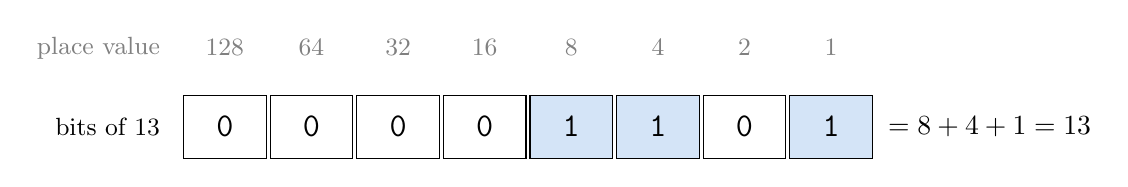
\begin{tikzpicture}[box/.style={draw,minimum width=1.05cm,minimum height=0.8cm,font=\large\ttfamily}]
  \foreach \v [count=\i] in {128,64,32,16,8,4,2,1} {
    \node[font=\small,gray] at (\i*1.1,1.0) {\v};
  }
  \foreach \b [count=\i] in {0,0,0,0,1,1,0,1} {
    \ifnum\b=1
      \node[box,fill=roba!20] at (\i*1.1,0) {\b};
    \else
      \node[box] at (\i*1.1,0) {\b};
    \fi
  }
  \node[anchor=west] at (9.4,0) {$= 8+4+1 = 13$};
  \node[anchor=east,font=\small,gray] at (0.4,1.0) {place value};
  \node[anchor=east,font=\small] at (0.4,0) {bits of 13};
\end{tikzpicture}
\caption{The number 13 as eight bits: \code{00001101}. The bits that are 1 sit under 8, 4 and 1,
and $8+4+1=13$.}
\end{figure}

A few more examples:
\[
  11 = \texttt{1011} = 8+2+1,\qquad 100 = \texttt{1100100} = 64+32+4,\qquad
  200 = \texttt{11001000} = 128+64+8.
\]

\paragraph{How many bits?} With 8 bits you can store $0$ to $255$; with one bit used for the sign,
$-127$ to $127$ (that is the \textbf{int8} type used by our networks). With 16 bits you can go up
to about $\pm 32{,}767$ (\textbf{int16}); with 32 bits up to about $\pm 2$ billion (\textbf{int32}).

\subsection{Shifting: the cheapest way to double}

If you write a 0 at the end of an everyday number, it becomes ten times bigger:
$13 \to 130$. In binary, writing a 0 at the end makes the number \emph{two} times bigger. Moving
all bits one place to the left is called a \textbf{left shift}, written \code{<<}.
\[
  13 = \texttt{1101}\quad\xrightarrow{\;<<1\;}\quad \texttt{11010} = 26,\qquad
  13 \ll 3 = \texttt{1101000} = 104 = 13\times 8.
\]
Shifting left by $k$ places multiplies by $2^k$. Shifting \emph{right} (\code{>>}) divides by
$2^k$ and throws away the remainder: $13 \gg 1 = \texttt{110} = 6$.

\begin{keyidea}
For a CPU, a shift costs \textbf{one clock cycle}, exactly like an addition. So multiplying by
1, 2, 4, 8, 16, \dots{} (a \emph{power of two}) is basically free. Multiplying by any other
number, like 11, is the hard part. All the tricks in this project are about turning hard
multiplications into shifts and additions.
\end{keyidea}

\subsection{Multiplying with only additions and shifts}\label{sec:shiftadd}

School multiplication works digit by digit. Binary multiplication works the same way, but every
digit is 0 or 1, so each step is either ``add a shifted copy'' or ``add nothing''.

\begin{example}[: $13\times 11$ by shift-and-add]
$11 = \texttt{1011}$. Look at the bits of 11 from the right. Each time, double 13; when the bit is 1,
add the current copy of 13 to the result.

\begin{center}
\begin{tabular}{cccccc}
\toprule
Step & bits of $b$ left & lowest bit & copy of $a$ & add? & result so far\\
\midrule
1 & \texttt{1011} & 1 & 13 & yes & 13\\
2 & \texttt{101}  & 1 & 26 & yes & 39\\
3 & \texttt{10}   & 0 & 52 & no  & 39\\
4 & \texttt{1}    & 1 & 104 & yes & \textbf{143}\\
\bottomrule
\end{tabular}
\end{center}
Indeed $13\times 11 = 143$. It took 4 rounds because 11 has 4 bits. An 8-bit number needs up to 8
rounds, a 16-bit number up to 16, a 31-bit number up to 31.
\end{example}

In C, the loop is only a few lines (this is Listing~1 of the paper, and the routine
\code{roba\_shift\_add} in our \file{csrc/roba\_core.h}):

\begin{lstlisting}[language=C]
uint32_t roba_shift_add(uint32_t a, uint32_t b)
{
    uint32_t r = 0;
    while (b) {           /* until no bits of b are left        */
        if (b & 1u)       /* lowest bit of b is 1?              */
            r += a;       /*   then add the current copy of a   */
        a <<= 1;          /* double a                           */
        b >>= 1;          /* drop the lowest bit of b           */
    }
    return r;
}
\end{lstlisting}

Each round runs about 6 instructions (test, branch, maybe add, two shifts, loop back), so an
exact 8-bit multiply costs tens of clock cycles, and it gets slower as numbers get bigger.
Our measurements later (Section~\ref{sec:multbench}) show 84 cycles for an 8-bit exact multiply
and 280 cycles for a 31-bit one.

\subsection{What a CPU is, and what a ``cycle'' is}

A \textbf{CPU} (processor) is the part of a chip that runs a program. A program is a long list of
very simple \textbf{instructions}, such as ``add these two numbers'', ``shift this number left by 3'',
``load a byte from memory'', ``if this is zero, jump over there''. The CPU keeps a few dozen
numbers close at hand in \textbf{registers} (32 of them on RISC-V, named \code{a0}, \code{a1},
\code{t0}, \dots).

The CPU is driven by a \textbf{clock}: a signal that ticks millions of times per second. One tick is
one \textbf{clock cycle}. A simple instruction like \code{add} takes one cycle; loading from memory
or a taken jump may take two or three.

\begin{example}[: from cycles to seconds]
If the chip's clock runs at 50~MHz (50 million ticks per second, a typical speed for a small
RISC-V core on an FPGA board), then one cycle lasts $1/50{,}000{,}000$~s $=20$~nanoseconds.
Our exact-multiply MLP needs 13.5 million cycles per image, i.e.\ $13.5\times 10^6 \times 20\,
\text{ns} = 0.27$~s per picture. With RoBA-Dn1 (7.05 million cycles) it is 0.14~s.
\end{example}

Because the clock speed depends on the chip, we always report \textbf{cycles}, not seconds.
Fewer cycles means faster \emph{and} (at the same power) less energy.

\subsection{RISC-V, Ibex, and why some chips have no multiplier}

\textbf{RISC-V} is a free, open \emph{instruction set}: a published list of which instructions a CPU
must understand. The base list, \textbf{RV32I}, has additions, shifts, logic, loads, stores and
jumps, but \textbf{no multiplication}. Multiplication is an optional add-on called the
\textbf{M extension}. Another add-on, \textbf{C}, adds short 16-bit versions of common
instructions to make programs smaller. Our CPU is \textbf{RV32IC}: base + compressed, no M.

\textbf{Ibex} is a small, real, open-source RISC-V CPU made by the company lowRISC. It is used in
real chips (for example in security chips) and can be built with or without a multiplier.

Why would anyone leave out the multiplier? A hardware multiplier is a big block of logic. The
paper synthesised Ibex for a 65~nm chip process and found that the multiplierless core with
the LOD instruction has \textbf{35.1\% less area}, a \textbf{10\% shorter critical path} (so it can
be clocked faster) and \textbf{17.1\% less power} than the same core with a single-cycle
multiplier. For a tiny battery-powered device, that is a lot.

\begin{kid}
A hardware multiplier is like a big, expensive kitchen machine. Many small kitchens don't
have room for it, so the cook does the job by hand. Hand work is slow. This project is about
finding a quick way of doing it by hand that is \emph{almost} as good as the machine.
\end{kid}

\subsection{The leading one, and the LOD instruction}\label{sec:lod}

The \textbf{leading one} of a number is its highest bit that is 1. Its \emph{position} (counting
from 0 at the right) tells you which power of two the number lies between:

\begin{center}
\begin{tabular}{rlcl}
\toprule
number & bits & leading-one position & so the number is between\\
\midrule
1 & \texttt{1} & 0 & $2^0=1$ and 2\\
13 & \texttt{1101} & 3 & $2^3=8$ and 16\\
11 & \texttt{1011} & 3 & 8 and 16\\
100 & \texttt{1100100} & 6 & 64 and 128\\
200 & \texttt{11001000} & 7 & 128 and 256\\
\bottomrule
\end{tabular}
\end{center}

\textbf{LOD} (``leading-one detector'') is the new instruction from the paper:
\[
  \texttt{lod rd, rs1}\qquad\Longrightarrow\qquad \texttt{rd} \gets \text{position of the leading 1 of } \texttt{rs1}.
\]
For example, if register \code{a1} holds 13, then \code{lod a0, a1} puts 3 into \code{a0}.
Then \code{1 << 3} $=8$ is the largest power of two that is not bigger than 13.

\paragraph{Why not do it in software?} Without the instruction, finding the leading one needs a
loop or a sequence of tests and shifts. On our core, the compiler's software version
(\code{\_\_clzsi2} in libgcc) makes RoBA-Dn1 cost \textbf{91 cycles} per multiply, which is slower
than the exact 84 cycles. With the LOD instruction it costs \textbf{28 cycles}
(Section~\ref{sec:multbench}). Without the new instruction, the whole idea does not pay off.

\paragraph{Why is it cheap in hardware?} In hardware, LOD is a \emph{priority encoder}: a small
circuit that looks at all 32 bits at once and outputs the position of the highest 1. It needs no
memory and no clock cycles of its own. It fits inside the existing arithmetic unit and answers in one
cycle, like an addition. The paper measured that it adds only \textbf{4.5\% power} to the
multiplierless core. Section~\ref{sec:lodpatch} shows the exact lines we added to Ibex.

\begin{keyidea}
LOD answers ``roughly how big is this number?'' in one cycle. Knowing the nearest power of two
of each number turns a multiplication into a few shifts and additions.
\end{keyidea}
\newpage

\section{Approximate multiplication: the eight multipliers}\label{sec:mult}

\subsection{The trick behind RoBA}

\textbf{RoBA} stands for \emph{Rounding-Based Approximate} multiplication. The idea:
\begin{enumerate}
  \item Round each number to a power of two: $a \to \Ar = 2^{p_a}$, $b \to \Br = 2^{p_b}$.
        (LOD gives $p_a$ and $p_b$ in one cycle each.)
  \item Multiplying by a power of two is a shift, so $\Ar\cdot b$, $a\cdot\Br$ and $\Ar\cdot\Br$ are all
        cheap.
  \item Use them to build an answer close to $a\cdot b$.
\end{enumerate}

Why is that possible? Write $a = \Ar + (a-\Ar)$ and $b = \Br + (b-\Br)$ and multiply out:
\[
  a\cdot b \;=\; \underbrace{\Ar\, b + a\,\Br - \Ar\Br}_{\text{all shifts: cheap}}
  \;+\; \underbrace{(a-\Ar)(b-\Br)}_{\text{the hard leftover}}.
\]
RoBA keeps the cheap part and \emph{drops the leftover}. The leftover is the product of two
small ``remainders'', so it is usually small compared with $a\cdot b$.

\begin{figure}[H]
\centering
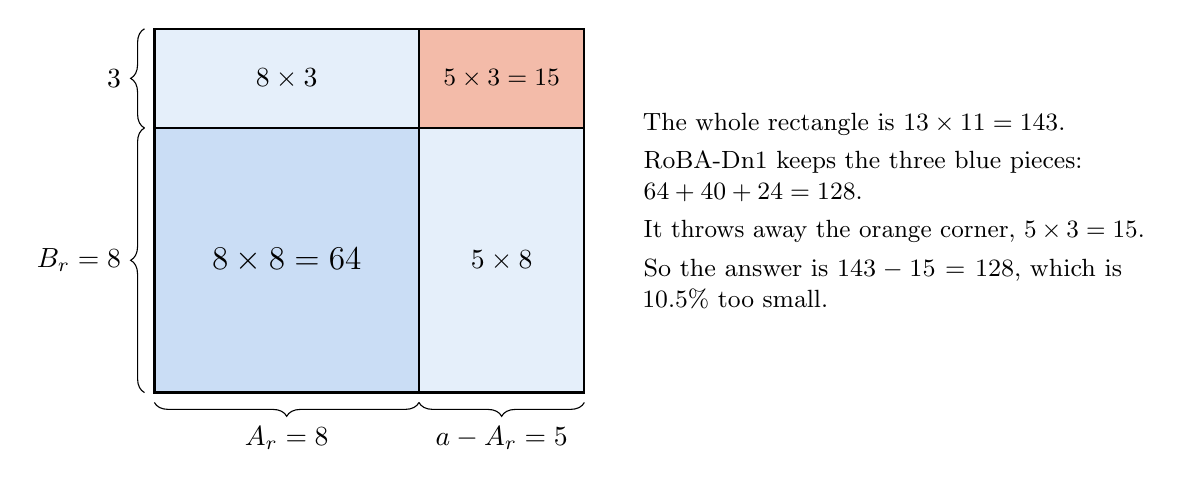
\begin{tikzpicture}[scale=0.42]
  % a = 13 (x), b = 11 (y); Ar = Br = 8
  \fill[roba!25] (0,0) rectangle (8,8);
  \fill[roba!12] (8,0) rectangle (13,8);
  \fill[roba!12] (0,8) rectangle (8,11);
  \fill[twoit!45] (8,8) rectangle (13,11);
  \draw[thick] (0,0) rectangle (13,11);
  \draw (8,0) -- (8,11); \draw (0,8) -- (13,8);
  \node at (4,4) {\large $8\times8=64$};
  \node at (10.5,4) {$5\times 8$};
  \node at (4,9.5) {$8\times 3$};
  \node[font=\small] at (10.5,9.5) {$5\times3=15$};
  \draw[decorate,decoration={brace,amplitude=5pt,mirror}] (0,-0.3) -- (8,-0.3) node[midway,below=5pt] {$\Ar=8$};
  \draw[decorate,decoration={brace,amplitude=5pt,mirror}] (8,-0.3) -- (13,-0.3) node[midway,below=5pt] {$a-\Ar=5$};
  \draw[decorate,decoration={brace,amplitude=5pt}] (-0.3,0) -- (-0.3,8) node[midway,left=5pt] {$\Br=8$};
  \draw[decorate,decoration={brace,amplitude=5pt}] (-0.3,8) -- (-0.3,11) node[midway,left=5pt] {$3$};
  \node[anchor=west,text width=6.3cm,font=\small] at (14.5,5.5) {%
    The whole rectangle is $13\times 11 = 143$.\\[3pt]
    RoBA-Dn1 keeps the three blue pieces:\\ $64 + 40 + 24 = 128$.\\[3pt]
    It throws away the orange corner, $5\times 3 = 15$.\\[3pt]
    So the answer is $143 - 15 = 128$, which is 10.5\% too small.};
\end{tikzpicture}
\caption{A product is the area of a rectangle. RoBA cuts the rectangle where the powers of two
are and drops the small corner piece.}
\label{fig:rect}
\end{figure}

\begin{example}[: RoBA-Dn1 on $13\times 11$]
LOD(13) = 3 and LOD(11) = 3, so $\Ar = \Br = 8$.
\[
  \Ar b + a\Br - \Ar\Br = (11\ll 3) + (13\ll 3) - (1\ll 6) = 88 + 104 - 64 = 128.
\]
Only three shifts, one addition and one subtraction. The true answer is 143.
\end{example}

\subsection{Rounding down or to the nearest power of two}

There are two ways to round to a power of two:
\begin{itemize}
  \item \textbf{Down (``Dn'')}: always the power of two just below (or equal): 13 $\to$ 8,
        11 $\to$ 8. That is exactly \code{1 << LOD(x)}.
  \item \textbf{Up-or-down (``UpDn'')}: the \emph{nearest} power of two. The rule is very cheap: look
        at the bit right after the leading one. If it is 1, the number is at least $1.5\times$ its
        lower power of two, so round up.
        $13 = \texttt{1\underline{1}01}$: the next bit is 1, so $13\to 16$.
        $11 = \texttt{1\underline{0}11}$: the next bit is 0, so $11\to 8$.
\end{itemize}

\begin{example}[: RoBA-UpDn on $13\times 11$]
$\Ar = 16$ ($p_a=4$), $\Br = 8$ ($p_b=3$).
\[
  (11\ll 4) + (13\ll 3) - (1\ll 7) = 176 + 104 - 128 = 152.
\]
That is 6.3\% \emph{too big}. Here the dropped corner is $(13-16)(11-8) = (-3)(3) = -9$, a
\emph{negative} piece, so dropping it makes the answer too large: $143-(-9) = 152$.
\end{example}

\begin{keyidea}
Rounding \emph{down} always gives an answer that is too small (the dropped corner is never
negative). Rounding to the \emph{nearest} power of two is sometimes too big and sometimes too small,
so on average the errors cancel out. This difference matters for neural networks
(Section~\ref{sec:whyok}).
\end{keyidea}

\subsection{Two-step versions: also estimate the corner}

The dropped corner $(a-\Ar)(b-\Br)$ is itself a multiplication of two (smaller) numbers. So we can
estimate it with RoBA \emph{again}, and add it back. That gives three more methods:

\begin{itemize}
  \item \textbf{RoBA-Dn2}: round down, then estimate the corner with Dn1.
  \item \textbf{RoBA-UpDnDn}: round to nearest, then estimate the (signed) corner with Dn1.
  \item \textbf{RoBA-(UpDn)2}: round to nearest, then estimate the corner with UpDn.
\end{itemize}

\begin{example}[: the two-step versions on $13\times 11$]
\textbf{Dn2.} First step as Dn1: 128. The corner is $5\times 3$. Dn1 on $5\times 3$:
LOD(5)=2, LOD(3)=1, so $(3\ll 2) + (5\ll 1) - (1\ll 3) = 12+10-8 = 14$ (true: 15).
Answer: $128 + 14 = \mathbf{142}$ ($-0.7\%$).

\textbf{UpDnDn.} First step as UpDn: 152. The corner is $(-3)\times 3$: the signs differ, so the
corner is negative. Dn1 on $3\times 3$: $(3\ll1)+(3\ll1)-(1\ll2) = 6+6-4 = 8$ (true: 9).
Answer: $152 - 8 = \mathbf{144}$ ($+0.7\%$).

\textbf{(UpDn)2.} Same, but UpDn on $3\times 3$: $3=\texttt{11}$, the next bit is 1, so it rounds up
to 4: $(3\ll2)+(3\ll2)-(1\ll4) = 12+12-16 = 8$. Answer: $152-8 = \mathbf{144}$.
\end{example}

The two-step versions are far more accurate, but each runs RoBA twice plus extra sign
handling, so they cost more cycles.

\subsection{The two older methods we compare against}

\paragraph{Mitchell (1962).} Mitchell's method works with logarithms: $\log_2(a\cdot b) =
\log_2 a + \log_2 b$, and it approximates $\log_2 a \approx p_a + (a-\Ar)/\Ar$. Turned into
integer steps (as in our code):
\[
  m = (a-\Ar)\Br + (b-\Br)\Ar,\quad p = \Ar\Br,\qquad
  \text{result} = \begin{cases} p + m & \text{if } m < p\\ 2m & \text{otherwise (a ``carry'')}.\end{cases}
\]
When $m<p$ this is exactly the same as RoBA-Dn1 ($p+m = \Ar b + a\Br - \Ar\Br$). The two differ only
in the carry case.
\begin{example}[: Mitchell]
$13\times 11$: $m = 5\cdot 8 + 3\cdot 8 = 64$, $p=64$, so $m\ge p$ and the result is $2m=128$, the same
as Dn1. $7\times 7$: $\Ar=\Br=4$, $m=3\cdot4+3\cdot4=24$, $p=16$, so the result is $2\cdot 24 = 48$
(true: 49). Dn1 gives $16+24=40$ here.
\end{example}
(The paper's ``Mitchell'', following Babi\'c et al., has no carry and gives exactly the same
products as RoBA-Dn1. Ours is the classic version with the carry.)

\paragraph{DRUM6.} DRUM keeps only the 6 most important bits of each number, starting at the
leading one, and forces the lowest kept bit to 1 (this makes the error unbiased on average). Then
it multiplies the two small 6-bit numbers \emph{exactly} and shifts the result back. Numbers below
64 are kept exact.
\begin{example}[: DRUM6 on $200\times 150$]
$200 = \texttt{110010|00}$: keep \texttt{110010}, set the last bit: \texttt{110011} $=51$; 2 bits
were cut, so it stands for $51\times 4 = 204$.
$150 = \texttt{100101|10}$: keep \texttt{100101} $=37$ (already ends in 1); it stands for
$37\times 4 = 148$. Then $51\times 37 = 1887$ (a small exact multiply), shifted back by $2+2=4$:
$1887\times 16 = 30192$. True: 30000, so $+0.64\%$.
\end{example}
DRUM6 is accurate, but on a multiplierless CPU the $6\times6$ ``small exact multiply'' is still a
shift-and-add loop, which makes it slow (we will see it is even slower than exact).

\subsection{All eight on two examples}

\begin{table}[H]
\centering
\small
\begin{tabular}{lrrrr}
\toprule
 & \multicolumn{2}{c}{$13\times 11 = 143$} & \multicolumn{2}{c}{$200\times 150 = 30000$}\\
\cmidrule(lr){2-3}\cmidrule(lr){4-5}
Multiplier & result & error & result & error\\
\midrule
Exact & 143 & 0 & 30000 & 0\\
Mitchell & 128 & $-10.5\%$ & 28416 & $-5.28\%$\\
DRUM6 & 143 & 0 (small numbers stay exact) & 30192 & $+0.64\%$\\
RoBA-Dn1 & 128 & $-10.5\%$ & 28416 & $-5.28\%$\\
RoBA-UpDn & 152 & $+6.3\%$ & 31232 & $+4.11\%$\\
RoBA-Dn2 & 142 & $-0.7\%$ & 29952 & $-0.16\%$\\
RoBA-UpDnDn & 144 & $+0.7\%$ & 30144 & $+0.48\%$\\
RoBA-(UpDn)2 & 144 & $+0.7\%$ & 29952 & $-0.16\%$\\
\bottomrule
\end{tabular}
\caption{Every value in this table was checked with the project's reference code
(\file{roba/reference.py}).}
\end{table}

\paragraph{Negative numbers.} All methods work on the sizes (absolute values) of the numbers, and the
sign is fixed at the end: $(-13)\times 11 \to 13\times 11 \approx 128 \to -128$. Two negatives give a
positive. This is called the \emph{sign-magnitude} approach.

\subsection{How wrong are they, on average?}\label{sec:errors}

We multiplied 1 million random pairs of 8-bit numbers with each method and measured the error
relative to the true product (\file{experiments/run.py}, stage \code{errors};
\file{results/*/multiplier\_errors.csv}).

\begin{figure}[H]
\centering
\includegraphics[width=\linewidth]{errors}
\caption{Left: the average and the worst error of each multiplier (8-bit operands). Right: the
average \emph{signed} error. Rounding down (Mitchell, Dn1, Dn2) is always too small, so the bar points
left. UpDn, UpDnDn and (UpDn)2 are centred on zero.}
\label{fig:errors}
\end{figure}

\begin{table}[H]
\centering
\small
\begin{tabular}{lrrrr}
\toprule
Multiplier & average error & worst error & average signed error & exactly right\\
\midrule
Mitchell & 3.79\% & 11.1\% & $-3.79\%$ & 6.2\%\\
DRUM6 & 1.30\% & 6.3\% & $+0.57\%$ & 14.0\%\\
RoBA-Dn1 & 8.92\% & 24.8\% & $-8.92\%$ & 6.2\%\\
RoBA-UpDn & 2.86\% & 11.1\% & $-0.01\%$ & 6.2\%\\
RoBA-Dn2 & 0.83\% & 6.1\% & $-0.83\%$ & 26.2\%\\
RoBA-UpDnDn & 0.24\% & 2.6\% & $-0.002\%$ & 39.7\%\\
RoBA-(UpDn)2 & 0.07\% & 0.8\% & $-0.0002\%$ & 39.7\%\\
\bottomrule
\end{tabular}
\caption{Error statistics over 1 million random pairs of 8-bit numbers. ``Exactly right'' is the
share of pairs where the method gives the exact product (for example when a number is already a
power of two).}
\end{table}

\begin{example}[: the worst case of Dn1]
Dn1 is worst when both numbers are just below the next power of two, so the dropped corner is as
big as possible. $255\times 255 = 65025$: $\Ar=\Br=128$, the corner is $127\times127 = 16129$, and
Dn1 gives $65025-16129 = 48896$, which is $24.8\%$ too small.
\end{example}

The picture below shows the error for every pair $a,b$ from 1 to 63. Each little square is one
multiplication; red means too small, blue means too big, white means (almost) exact. The thin lines
are at the powers of two, where the pattern restarts.

\begin{figure}[H]
\centering
\includegraphics[width=\linewidth]{error_map}
\caption{Error of $a\times b$ for $a,b = 1\dots63$. Dn1 is never too big (only red); its error grows
towards the top-right of each square between powers of two. UpDn has red and blue, which cancel.
(UpDn)2 is almost white everywhere.}
\end{figure}

\subsection{How the multipliers look in code}

All eight exist three times, and tests check that the three agree on every product:
\begin{itemize}
  \item in PyTorch, for fast GPU experiments (\file{roba/multipliers.py});
  \item in plain Python bit operations, as an independent reference (\file{roba/reference.py});
  \item in C, for the Ibex CPU (\file{csrc/roba.c}, and the inline copy \file{csrc/roba\_core.h}).
\end{itemize}

Here is the C version of the two one-step RoBA methods (from \file{csrc/roba\_core.h}). Compare it
with the formulas above:

\begin{lstlisting}[language=C]
/* Leading-one position, rounded up when the next bit is set (nearest power of two). */
static inline uint32_t pos_updn(uint32_t x)
{
    uint32_t p = LOD(x);                       /* one LOD instruction            */
    if (p > 0 && ((x >> (p - 1)) & 1u))        /* bit after the leading one = 1? */
        p++;                                   /*   then round up                */
    return p;
}

/* Ar*b + a*Br - Ar*Br, all as shifts: (b << pa) + (a << pb) - (1 << (pa+pb)) */
static inline uint32_t roba1(uint32_t a, uint32_t b, uint32_t pa, uint32_t pb)
{
    return (b << pa) + (a << pb) - ((1u << pa) << pb);
}

static inline uint32_t roba_dn1_nz(uint32_t a, uint32_t b)  { return roba1(a, b, LOD(a), LOD(b)); }
static inline uint32_t roba_updn_nz(uint32_t a, uint32_t b) { return roba1(a, b, pos_updn(a), pos_updn(b)); }
\end{lstlisting}

The suffix \code{\_nz} means ``non-zero'': the caller has already checked that neither number is 0
(LOD of 0 has no meaningful answer, and anything times 0 is 0 anyway).
\newpage

\section{Neural networks, from zero}\label{sec:nn}

\subsection{One neuron}

A \textbf{neuron} takes some numbers in, multiplies each by its own \textbf{weight}, adds everything
up, adds one more number called the \textbf{bias}, and passes the result through a simple rule
called \textbf{ReLU}: negative numbers become 0, positive numbers stay as they are.
\[
  \text{output} = \text{ReLU}\Big(\sum_k x_k\,w_k + b\Big),\qquad \text{ReLU}(v) = \max(v, 0).
\]
Each $x_k w_k$ is one multiplication, and adding it to the running sum is one
\textbf{multiply-accumulate}, or \textbf{MAC}. MACs are almost all the work a network does.

\begin{figure}[H]
\centering
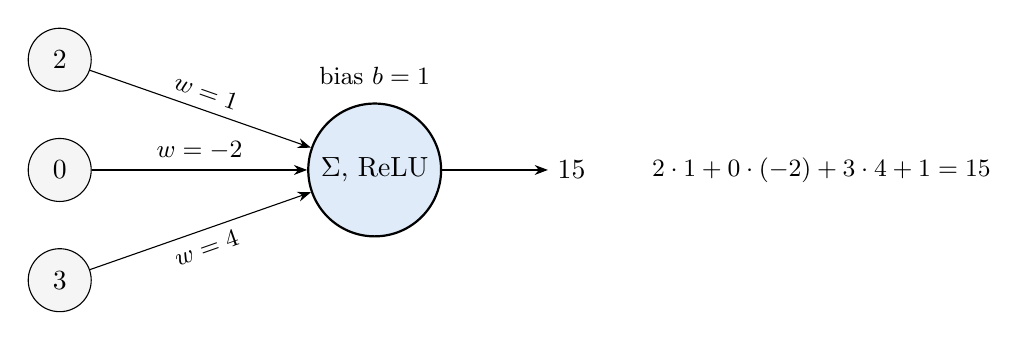
\begin{tikzpicture}[>=Stealth,node distance=1.0cm,
  inp/.style={circle,draw,minimum size=0.8cm,fill=gray!8},
  neu/.style={circle,draw,thick,minimum size=1.3cm,fill=roba!15}]
  \node[inp] (x1) at (0,1.4) {2};
  \node[inp] (x2) at (0,0) {0};
  \node[inp] (x3) at (0,-1.4) {3};
  \node[neu] (n) at (4,0) {$\Sigma$, ReLU};
  \draw[->] (x1) -- node[above,sloped,font=\small] {$w=1$} (n);
  \draw[->] (x2) -- node[above,font=\small] {$w=-2$} (n);
  \draw[->] (x3) -- node[below,sloped,font=\small] {$w=4$} (n);
  \node[above=0.1cm of n,font=\small] {bias $b=1$};
  \draw[->] (n) -- ++(2.2,0) node[right] {15};
  \node[font=\small,anchor=west] at (7.4,0) {$2\cdot1 + 0\cdot(-2) + 3\cdot 4 + 1 = 15$};
\end{tikzpicture}
\caption{One neuron with three inputs. It does three multiplications. If the weights were
$(-3,1,1)$ and the bias 0, the sum would be $-6+0+3=-3$, and ReLU would output 0.}
\end{figure}

\begin{kid}
A neuron is like a judge giving points. Each clue (input) has an importance (weight). The judge adds
up \emph{clue $\times$ importance} for all clues. If the total is negative, the judge says ``nothing'' (0).
\end{kid}

\subsection{Layers, scores and the answer}

A \textbf{layer} is many neurons that all look at the same inputs. The outputs of one layer are the
inputs of the next. The last layer has one neuron per possible answer (10 here: the digits 0--9, or 10
kinds of clothes). Its outputs are called \textbf{scores} or \textbf{logits}, and the network's answer is
the class with the \emph{largest} score (``argmax'').

\begin{example}[: from scores to an answer, and the loss]
Suppose the scores for three classes are $(2,1,0)$. The answer is class 0. During training, scores are
turned into probabilities with \emph{softmax}: $e^2=7.39$, $e^1=2.72$, $e^0=1$, total $11.1$, so the
probabilities are $0.665, 0.245, 0.090$. If class 0 is correct, the \textbf{loss} is
$-\ln 0.665 = 0.41$. If the network were sure (probability 1), the loss would be 0. The loss measures how
``surprised'' the network is by the right answer. Training changes the weights to make the loss small.
\end{example}

\textbf{Training} means: show the network many pictures with the right answers, compute the loss, and
nudge every weight a tiny bit in the direction that lowers the loss (the direction is found by
\emph{backpropagation}; the nudging rule we use is called \emph{Adam}). One pass over all training
pictures is an \textbf{epoch}. \textbf{Test accuracy} is the share of \emph{new} pictures (never seen
in training) that the network gets right.

\subsection{The two datasets}

\begin{itemize}
  \item \textbf{MNIST}: 70{,}000 hand-written digits (0--9), each $28\times 28$ grey pixels; 60{,}000 for
        training and 10{,}000 for testing. Easy: good networks get about 99\%.
  \item \textbf{Fashion-MNIST}: the same size and format, but the 10 classes are T-shirt, trouser,
        pullover, dress, coat, sandal, shirt, sneaker, bag and ankle boot. Harder (about 90\%), because
        a shirt and a pullover can look very alike.
\end{itemize}

Each pixel is a number from 0 (black) to 255 (white). Before the network sees it, it is divided by 255
and then \textbf{normalised}: $x = (p/255 - \text{mean})/\text{std}$, with mean $0.1307$ and std
$0.3081$ for MNIST (mean $0.2860$, std $0.3530$ for Fashion-MNIST). Normalising keeps the numbers centred
around 0, which makes training easier.

\begin{example}[: normalising a pixel]
For MNIST, a black pixel ($p=0$) becomes $(0-0.1307)/0.3081 = -0.424$ and a white pixel ($p=255$)
becomes $(1-0.1307)/0.3081 = 2.82$. Note that black is \textbf{not zero} after normalising. This will
matter a lot in Section~\ref{sec:zeroskip}.
\end{example}

\subsection{Network 1: the MLP}

An \textbf{MLP} (multi-layer perceptron) is the simplest network: layers in which every neuron sees
every input (``fully connected'', FC). Ours flattens the $28\times28$ picture into 784 numbers and uses
three layers:
\[
  784 \xrightarrow{\text{FC}} 256 \xrightarrow{\text{ReLU, FC}} 128 \xrightarrow{\text{ReLU, FC}} 10.
\]

\begin{example}[: how many multiplications does the MLP do?]
Every neuron multiplies each of its inputs once:
\[
  784\times256 + 256\times128 + 128\times10 = 200{,}704 + 32{,}768 + 1{,}280 = \mathbf{234{,}752}
\]
multiplications per picture. 85\% of them are in the first layer.
\end{example}

\subsection{Network 2: LeNet-5, with convolutions}

A \textbf{convolution} layer slides a small grid of weights (a \textbf{filter}, here $5\times5$) over
the picture. At every position, it multiplies the 25 pixels under the filter by the 25 weights and adds
them up. The same filter is used everywhere, so it finds the same pattern (an edge, a curve) wherever it
appears.

\begin{example}[: a $3\times3$ filter that finds vertical edges]
Filter $\begin{pmatrix}1&0&-1\\1&0&-1\\1&0&-1\end{pmatrix}$.
On a patch with a bright left part and a dark right part,
$\begin{pmatrix}9&9&0\\9&9&0\\9&9&0\end{pmatrix}$, the result is $9+9+9-0-0-0 = 27$: an edge.
On a flat patch $\begin{pmatrix}9&9&9\\9&9&9\\9&9&9\end{pmatrix}$, the result is
$27-27 = 0$: no edge. Each position costs 9 multiplications.
\end{example}

\textbf{Max pooling} ($2\times2$) shrinks a picture by keeping the biggest of every 4 neighbours, e.g.
$\begin{pmatrix}1&3\\2&0\end{pmatrix}\to 3$. It has no multiplications.

\begin{figure}[H]
\centering
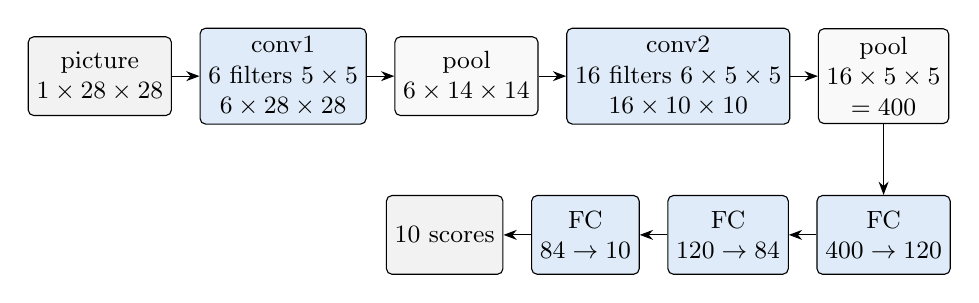
\begin{tikzpicture}[>=Stealth,font=\small,
  blk/.style={draw,rounded corners=2pt,align=center,minimum height=1.0cm,inner sep=3pt}]
  \node[blk,fill=gray!10] (in) {picture\\$1\times28\times28$};
  \node[blk,fill=roba!15,right=0.35cm of in] (c1) {conv1\\6 filters $5\times5$\\$6\times28\times28$};
  \node[blk,fill=gray!5,right=0.35cm of c1] (p1) {pool\\$6\times14\times14$};
  \node[blk,fill=roba!15,right=0.35cm of p1] (c2) {conv2\\16 filters $6\times5\times5$\\$16\times10\times10$};
  \node[blk,fill=gray!5,right=0.35cm of c2] (p2) {pool\\$16\times5\times5$\\$=400$};
  \node[blk,fill=roba!15,below=0.9cm of p2] (f1) {FC\\$400\to120$};
  \node[blk,fill=roba!15,left=0.35cm of f1] (f2) {FC\\$120\to84$};
  \node[blk,fill=roba!15,left=0.35cm of f2] (f3) {FC\\$84\to10$};
  \node[blk,fill=gray!10,left=0.35cm of f3] (out) {10 scores};
  \draw[->] (in) -- (c1); \draw[->] (c1) -- (p1); \draw[->] (p1) -- (c2); \draw[->] (c2) -- (p2);
  \draw[->] (p2) -- (f1); \draw[->] (f1) -- (f2); \draw[->] (f2) -- (f3); \draw[->] (f3) -- (out);
\end{tikzpicture}
\caption{LeNet-5 as used here (ReLU after every layer except the last).}
\end{figure}

\begin{example}[: how many multiplications does LeNet-5 do?]
\begin{tabular}{@{}ll@{}}
conv1: & 6 filters $\times$ $28\times28$ positions $\times$ 25 weights $= 117{,}600$\\
conv2: & 16 filters $\times$ $10\times10$ positions $\times$ $(6\times25=150)$ weights $= 240{,}000$\\
FC layers: & $400\times120 + 120\times84 + 84\times10 = 48{,}000+10{,}080+840 = 58{,}920$\\
total: & $\mathbf{416{,}520}$ multiplications per picture.
\end{tabular}
\end{example}

\begin{inthecode}{roba/nn.py}
\code{class MLP} and \code{class LeNet5} define the two networks. Their layers are \code{ALinear} and
\code{AConv2d}: normal PyTorch layers whose multiplications can be switched to any of our eight
multipliers and any number format (``domain'').
\end{inthecode}

\subsection{Turning decimals into whole numbers: quantization}\label{sec:quant}

A trained network's weights are decimals like $0.2$ or $-0.0371$. Our small CPU has no hardware for
decimals (no floating-point unit), and the approximate multipliers work on whole numbers anyway. So we
\textbf{quantize}: represent every decimal as a whole number times a fixed \emph{scale}.

For 8 bits (\textbf{int8}), the whole numbers go from $-127$ to $127$:
\begin{itemize}
  \item Weights: for each output neuron, $s_w = \max|w| / 127$ and $w_{\text{int}} = \text{round}(w/s_w)$.
  \item Activations (layer inputs): $s_x = (\text{largest input seen on 5{,}000 training pictures})/127$
        and $x_{\text{int}} = \text{round}(x/s_x)$.
  \item Then $\sum x_k w_k \approx s_x s_w \sum x_{\text{int},k}\, w_{\text{int},k}$. The sum is
        made of whole-number products, which is what the approximate multipliers compute.
\end{itemize}

\begin{example}[: quantizing one product]
Say the largest weight of a neuron is $0.5$, so $s_w = 0.5/127 = 0.003937$. A weight $w=0.2$ becomes
$\text{round}(0.2/0.003937) = \text{round}(50.8) = 51$.
Say the largest input is $4.0$, so $s_x = 4/127 = 0.0315$. An input $x=1.3$ becomes
$\text{round}(41.3) = 41$.
The integer product is $41\times 51 = 2091$, and $2091\times s_x s_w = 2091\times 0.000124 = 0.2593$.
The true product is $1.3\times0.2 = 0.26$. Very close.
\end{example}

\begin{careful}
Simply cutting decimals to integers \emph{without} a scale (``trunc'') destroys the network:
$\text{trunc}(0.2) = 0$, and nearly every weight is between $-1$ and $1$, so nearly every weight
becomes 0. The network then always gives the same answer and gets about \textbf{10\%}, the same as
guessing (Figure~\ref{fig:domains}). We kept this case in the results to show why scaling is needed.
\end{careful}

We also tried \textbf{int16} ($-32767\dots32767$), which is more precise. For these networks it gives
the same accuracy as int8, so the Ibex part uses int8.

\subsubsection*{Integer-only rescaling (what the CPU actually does)}

After a layer adds up its integer products into \code{acc}, the next layer needs its input as int8
again, with its own scale $s_{\text{next}}$. On the GPU we just multiply by
$s_x s_w/s_{\text{next}}$. On Ibex there are no decimals, so we use \textbf{fixed point}: store the
decimal scale as a whole number $M$ that is $2^{24}$ times bigger, and shift right by 24 at the end.
\[
  M = \text{round}\Big(\frac{s_x s_w}{s_{\text{next}}}\cdot 2^{24}\Big),\quad
  C = \text{round}\Big(\frac{b}{s_{\text{next}}}\cdot 2^{24}\Big),\quad
  y = \big(\texttt{acc}\cdot M + C + 2^{23}\big) \gg 24.
\]
The $2^{23}$ (half of $2^{24}$) makes the shift \emph{round} instead of cutting off. Then ReLU and a
clamp to $0\dots127$ give the next layer's int8 input.

\begin{example}[: one rescale, step by step]
Take $\texttt{acc} = 2091$, a scale $s_xs_w/s_{\text{next}} = 0.0025$ and a bias that is worth $1.5$
in the next layer's units.
\begin{itemize}
  \item $M = \text{round}(0.0025\times 16{,}777{,}216) = \text{round}(41{,}943.04) = 41{,}943$.
  \item $C = 1.5\times16{,}777{,}216 = 25{,}165{,}824$.
  \item $2091\times 41{,}943 = 87{,}702{,}813$, plus $C$, plus $2^{23} = 8{,}388{,}608$, gives
        $121{,}257{,}245$.
  \item $121{,}257{,}245 \gg 24 = \lfloor 121{,}257{,}245 / 16{,}777{,}216\rfloor = \lfloor 7.23\rfloor = 7$.
\end{itemize}
Check with decimals: $2091\times0.0025 + 1.5 = 6.73$, which rounds to 7. The same answer, using only
whole numbers.
\end{example}

The $\texttt{acc}\cdot M$ product is done \emph{exactly} (with a shift-and-add loop), but only once per
neuron: 394 times per picture for the MLP, against 234{,}752 MACs. It is under 1\% of the time.

\begin{inthecode}{hw/run\_ibex.py and hw/sw/dnn.c}
\code{int\_model()} in \file{hw/run\_ibex.py} turns a trained PyTorch checkpoint into int8 weights
\code{W}, multipliers \code{M} and offsets \code{C} (with \code{SH = 24}) and writes them into a C header
\file{model.h}. \code{rescale()} and \code{relu\_q()} in \file{hw/sw/dnn.c} do the formula above on the CPU.
\end{inthecode}

\subsection{Running approximate multipliers fast on a GPU}\label{sec:factors}

A GPU is very fast at \emph{exact} matrix multiplication (many MACs at once), but it has no instruction
for ``RoBA-multiply''. Doing 10{,}000 test pictures $\times$ 400{,}000 products one by one in Python
would take far too long. The trick (in \file{roba/multipliers.py} and \file{roba/matmul.py}): every
RoBA method can be rewritten as a sum of a few \emph{exact} products of per-number pieces. For Dn1:
\[
  \text{Dn1}(x,w) = \Ar(x)\cdot w + \big(x-\Ar(x)\big)\cdot\Br(w),
\]
so a whole layer is two ordinary matrix multiplications:
$\Ar(X)\,W^{\mathsf T} + (X-\Ar(X))\,\Br(W)^{\mathsf T}$.

\begin{example}[: the piece trick on $13\times 11$]
$\Ar(13)\cdot 11 + (13-8)\cdot\Br(11) = 8\cdot 11 + 5\cdot 8 = 88+40 = 128$, the same as Dn1. A two-step
method just adds two more pieces. Only Mitchell (because of its ``if carry'' rule) cannot be split,
so it is computed element by element in chunks. That is why Mitchell's fine-tuning took about 4 times
longer than the others.
\end{example}

\subsection{Fine-tuning with the approximate multiplier}

After quantizing, we can also \textbf{fine-tune}: train a few more epochs (3 for MNIST, 5 for
Fashion-MNIST, with a small learning rate) while the network uses the approximate multiplier. The
forward pass uses the real approximate products. The backward pass (which computes how to change the
weights) pretends the multiplier is exact, because the approximate one has no usable slope. This
pretending is called the \emph{straight-through estimator}.

\begin{kid}
Fine-tuning is like practising with a slightly wrong calculator. After a while you learn how it is
wrong and adjust your own numbers so that the final answers come out right.
\end{kid}
\newpage

\section{Phase 1 results: accuracy on the GPU}\label{sec:gpu}

\subsection{What was run}

\file{experiments/run.py} runs four stages for each dataset on an NVIDIA L40 GPU:
\begin{enumerate}
  \item \textbf{errors}: the multiplier error statistics of Section~\ref{sec:errors}.
  \item \textbf{train}: normal float32 training of both networks (MNIST: 15 epochs, Fashion-MNIST:
        30 epochs; Adam, learning rate $10^{-3}$ with cosine decay, batch 128, seed 0).
  \item \textbf{eval}: every trained network in four number formats (float, trunc, int8, int16) times eight
        multipliers, on all 10{,}000 test pictures.
  \item \textbf{finetune}: for int8 and int16, a few more epochs with each multiplier, then evaluate again.
\end{enumerate}
The results are in \file{results/mnist/} and \file{results/fashion/} (\file{eval\_*.csv},
\file{finetune\_*.csv}, \file{multiplier\_errors.csv}).

\subsection{Number formats: scaling is essential}

\begin{figure}[H]
\centering
\includegraphics[width=0.85\linewidth]{domains}
\caption{Test accuracy with the exact multiplier in four number formats. Cutting decimals to
integers without a scale (``cut to int'') collapses to 10\%, which is guessing. int8 and int16 are as good
as float32.}
\label{fig:domains}
\end{figure}

\subsection{Accuracy with every multiplier}

\begin{figure}[H]
\centering
\includegraphics[width=\linewidth]{gpu_acc}
\caption{Test accuracy (10{,}000 test pictures) for int8 networks with each multiplier, before (solid) and
after (light) fine-tuning. The dashed line is the original float32 network. \textbf{Look at the
vertical axis}: each panel spans only about one percentage point, so the bars look more different than they
are.}
\label{fig:gpuacc}
\end{figure}

\begin{table}[H]
\centering
\small
\begin{tabular}{lcccccccc}
\toprule
 & \multicolumn{2}{c}{MNIST MLP} & \multicolumn{2}{c}{MNIST LeNet-5} & \multicolumn{2}{c}{Fashion MLP} &
   \multicolumn{2}{c}{Fashion LeNet-5}\\
\cmidrule(lr){2-3}\cmidrule(lr){4-5}\cmidrule(lr){6-7}\cmidrule(lr){8-9}
 & int8 & +FT & int8 & +FT & int8 & +FT & int8 & +FT\\
\midrule
float32 & \multicolumn{2}{c}{98.42} & \multicolumn{2}{c}{99.20} & \multicolumn{2}{c}{89.79} & \multicolumn{2}{c}{90.99}\\
\midrule
Exact & 98.43 & 98.43 & 99.18 & 99.21 & 89.82 & 89.77 & 90.95 & 90.88\\
Mitchell & 98.46 & 98.46 & 99.12 & 99.20 & 89.75 & 89.82 & 90.82 & 91.15\\
DRUM6 & 98.43 & 98.44 & 99.17 & 99.20 & 89.69 & 89.77 & 90.92 & 90.97\\
RoBA-Dn1 & 98.42 & 98.44 & 99.19 & 99.18 & 89.69 & 89.66 & \textbf{90.20} & 90.77\\
RoBA-UpDn & 98.44 & 98.42 & 99.20 & 99.22 & 89.89 & 89.74 & 90.72 & 90.84\\
RoBA-Dn2 & 98.44 & 98.51 & 99.20 & 99.21 & 89.74 & 89.71 & 90.91 & 91.01\\
RoBA-UpDnDn & 98.43 & 98.44 & 99.19 & 99.18 & 89.83 & 89.75 & 91.07 & 90.95\\
RoBA-(UpDn)2 & 98.44 & 98.47 & 99.21 & 99.19 & 89.77 & 89.73 & 90.98 & 90.97\\
\bottomrule
\end{tabular}
\caption{Test accuracy in \% (int8). ``+FT'' = after fine-tuning with that multiplier. The biggest
drop anywhere is RoBA-Dn1 on Fashion-MNIST LeNet-5: $90.95\to90.20$, i.e.\ $-0.75$ points, and
fine-tuning brings it back to 90.77.}
\label{tab:gpuacc}
\end{table}

\begin{careful}
We trained with one random seed. Training the same network twice with different seeds usually changes
accuracy by about 0.1 points, so differences smaller than that (most of this table) are noise, not a real
effect. ``Mitchell + FT is the best on Fashion LeNet-5'' is \emph{not} a real finding.
\end{careful}

\subsection{Why can a 9\%-wrong multiplier keep 99\% of the accuracy?}\label{sec:whyok}

RoBA-Dn1 is on average 8.9\% too small on every single multiplication, yet the networks barely notice.
Three reasons:

\paragraph{1. A consistent ``too small'' is like turning the volume down.} If every product in a sum is
about 9\% too small, the whole sum is about 9\% too small. The \emph{largest} score stays the largest.
\begin{example}[: shrinking all scores]
Scores $(5.0, 4.0, 1.0)$, answer: class 0. Multiply all by $0.91$: $(4.55, 3.64, 0.91)$, answer: still
class 0. It only goes wrong when two scores are nearly tied \emph{and} the bias (which is not shrunk)
tips the balance, which is rare. This is also why the loss of Dn1 is \emph{lower} than exact on Fashion
(0.376 vs 0.434 for the MLP): smaller scores make the network less over-confident when it is wrong.
\end{example}

\paragraph{2. Random errors cancel in a long sum.} A neuron in the MLP's first layer adds 784 products.
Errors that are sometimes positive and sometimes negative (UpDn, DRUM6) largely cancel out.
\begin{example}[: errors cancelling]
Four products whose true value is 100 each come out as $106, 96, 103, 95$ (errors $+6\%, -4\%,
+3\%, -5\%$). Their sum is $106+96+103+95 = 400$: exactly the true sum. Each one is up to 6\% wrong,
but together they are 0\% wrong. In general, the
relative error of a sum of $n$ independent errors shrinks about like $1/\sqrt{n}$: for $n=784$, about 28
times smaller.
\end{example}

\paragraph{3. Networks are robust by nature.} They are trained to recognise a shoe whether it is
slightly brighter, shifted or noisy. A small error in the arithmetic looks to them like a bit of noise.

\begin{keyidea}
Accuracy is \textbf{not} the problem: every multiplier stays within 0.75 points of exact, and most within
0.2 points. So the choice of multiplier should be made on \textbf{speed and energy}, which is what Phase~2
measures on the real CPU.
\end{keyidea}

\subsection{What the old cost estimate said}

Before measuring on Ibex, \file{roba/cost.py} estimated cycles by reading the cycles per multiply from
Fig.~4 of the paper (e.g.\ 8-bit: exact 44, Dn1 19) and multiplying by the number of MACs. Those
estimates are kept in the CSV files (\code{mult\_cycles}, \code{energy\_rel}) but are replaced by the
real measurements below. The measurements turned out higher than the estimates, because a real program
also spends time loading numbers, handling signs and looping, not only multiplying.
\newpage

\section{Phase 2 setup: the Ibex CPU and the LOD instruction}\label{sec:ibex}

\subsection{What exactly is simulated}

We did not have a physical chip yet (an FPGA board comes later). Instead, we ran the \emph{real hardware
description} of Ibex in a simulator:
\begin{itemize}
  \item \textbf{Ibex} is written in SystemVerilog, a language that describes circuits: wires, registers,
        adders, and how they are connected.
  \item \textbf{Verilator} translates that description into a C++ program that computes, clock tick by
        clock tick, exactly what every wire of the chip would do. This is called a
        \textbf{cycle-accurate} simulation: the cycle counts are the ones a real chip built from the same
        description would have.
  \item The \textbf{Simple System} is lowRISC's minimal test computer around Ibex: the CPU, 1~MB of
        memory (RAM that answers in one cycle), a timer, and a ``printer'' address. Characters written there
        appear in a log file (\file{ibex\_simple\_system.log}).
\end{itemize}

\begin{kid}
Verilator builds a perfect toy model of the chip inside the computer, so detailed that it moves every
little part once per tick. It is slow (about 1 million ticks per second, while a real chip does 50
million or more), but it never lies about how many ticks a program needs.
\end{kid}

\subsection{The configuration and the tools}

\begin{table}[H]
\centering
\small
\begin{tabularx}{\linewidth}{lX}
\toprule
Ibex version & lowRISC Ibex, fixed at commit \code{7b5df75} (the last one before a big rewrite), plus our
patch \file{hw/patches/0001-ibex-lod-instruction.patch}\\
CPU configuration & the ``small'' configuration, with the multiplier set to \code{RV32MNone}: the core
cannot run \code{mul} or \code{div}. Instruction set RV32IC + our LOD\\
Simulator & Verilator 4.228 (installed with conda, no administrator rights needed), FuseSoC to build\\
Compiler & lowRISC GCC 10.2 for RISC-V (\code{-march=rv32ic -O3}), bare metal (no operating system)\\
Memory & 960~kB for program and data plus a 32~kB stack (\file{hw/sw/link\_1mb.ld}); the int8 MLP weights
alone are 230~kB\\
Timing & the CPU's own cycle counter (\code{mcycle}), read before and after every picture and every
layer\\
Setup scripts & \file{hw/setup.sh} (tools, Ibex, patch), \file{hw/build\_sim.sh} (builds the simulator),
\file{hw/run\_sim.sh} (runs one program)\\
\bottomrule
\end{tabularx}
\caption{The Ibex setup.}
\end{table}

\begin{careful}
The compiler's helper library (libgcc) was built for a core \emph{with} a multiplier, so a few of its
helpers contain \code{mul}/\code{div} instructions, which would crash our core. Every time a program is
built, \file{hw/run\_ibex.py} (and \file{hw/sw/Makefile}) disassemble it and stop with an error if any
\code{mul}, \code{mulh}, \code{div} or \code{rem} instruction is found. The exact multiply in C
(\code{a * b}) becomes a call to libgcc's \code{\_\_mulsi3}, which is a shift-and-add loop: the
paper's baseline.
\end{careful}

\subsection{How LOD was added to Ibex}\label{sec:lodpatch}

A CPU handles every instruction in steps. Ibex has two main stages: \textbf{fetch} (read the instruction
from memory) and \textbf{decode/execute} (work out what the instruction means, read the registers, compute
in the ALU, write the result back). To add an instruction you must teach the \textbf{decoder} to recognise it
and give the \textbf{ALU} (arithmetic logic unit) a circuit that computes it.

\begin{figure}[H]
\centering
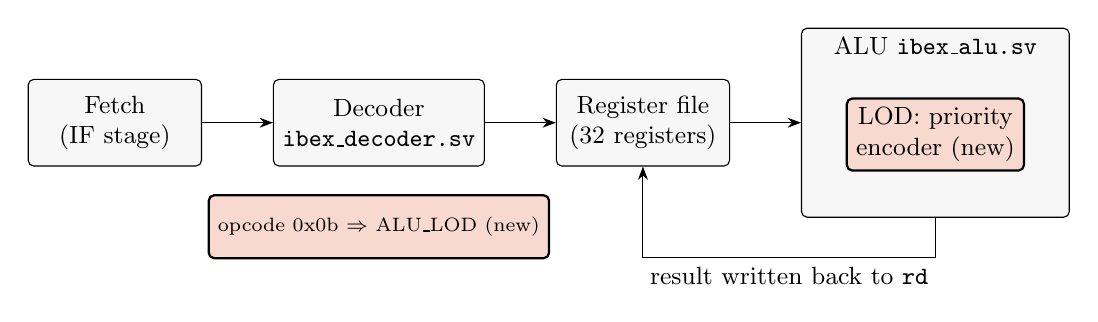
\begin{tikzpicture}[>=Stealth,font=\small,
  blk/.style={draw,rounded corners=2pt,align=center,minimum height=1.1cm,minimum width=2.2cm,fill=gray!6},
  new/.style={draw,thick,rounded corners=2pt,align=center,fill=twoit!25,minimum height=0.8cm}]
  \node[blk] (if) {Fetch\\(IF stage)};
  \node[blk,right=0.9cm of if] (dec) {Decoder\\\file{ibex\_decoder.sv}};
  \node[blk,right=0.9cm of dec] (rf) {Register file\\(32 registers)};
  \node[blk,right=0.9cm of rf,minimum width=3.4cm,minimum height=2.4cm] (alu) {};
  \node[anchor=north,font=\small] at (alu.north) {ALU \file{ibex\_alu.sv}};
  \node[new] (lod) at ($(alu.center)+(0,-0.15)$) {LOD: priority\\encoder (new)};
  \node[new,below=0.35cm of dec,font=\scriptsize] (dnew) {opcode 0x0b $\Rightarrow$ ALU\_LOD (new)};
  \draw[->] (if) -- (dec); \draw[->] (dec) -- (rf); \draw[->] (rf) -- (alu);
  \draw[->] (alu.south) -- ++(0,-0.5) -| node[pos=0.25,below] {result written back to \code{rd}} (rf.south);
\end{tikzpicture}
\caption{Where the patch touches Ibex. The orange parts are new; the rest of the core is unchanged.}
\end{figure}

\paragraph{Step 1: choose an encoding.} Every RISC-V instruction is a 32-bit number. The lowest 7 bits
(the \emph{opcode}) say which kind of instruction it is. RISC-V reserves opcode \code{0001011} (hex
\code{0x0b}, called \textbf{custom-0}) for exactly this purpose: vendors may put their own instructions
there, and no standard instruction will ever use it. LOD uses the standard ``R-type'' layout:

\begin{figure}[H]
\centering
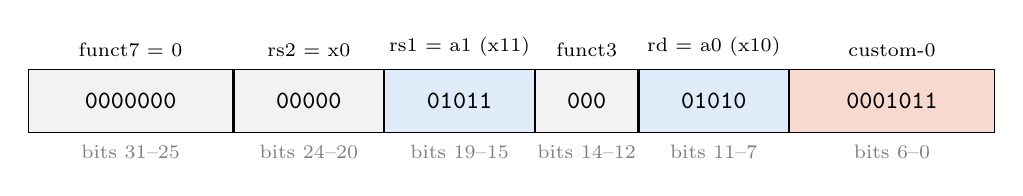
\begin{tikzpicture}[font=\small\ttfamily,
  f/.style={draw,minimum height=0.8cm,align=center}]
  \node[f,minimum width=2.6cm,fill=gray!10] (f7) at (0,0) {0000000};
  \node[f,minimum width=1.9cm,fill=gray!10,right=0pt of f7] (rs2) {00000};
  \node[f,minimum width=1.9cm,fill=roba!15,right=0pt of rs2] (rs1) {01011};
  \node[f,minimum width=1.3cm,fill=gray!10,right=0pt of rs1] (f3) {000};
  \node[f,minimum width=1.9cm,fill=roba!15,right=0pt of f3] (rd) {01010};
  \node[f,minimum width=2.6cm,fill=twoit!25,right=0pt of rd] (op) {0001011};
  \foreach \n/\t/\b in {f7/funct7 = 0/31--25, rs2/rs2 = x0/24--20, rs1/rs1 = a1 (x11)/19--15,
                        f3/funct3/14--12, rd/rd = a0 (x10)/11--7, op/custom-0/6--0} {
    \node[above=1pt of \n,font=\scriptsize\rmfamily] {\t};
    \node[below=1pt of \n,font=\scriptsize\rmfamily,gray] {bits \b};
  }
\end{tikzpicture}
\caption{The 32 bits of \code{lod a0, a1}. As one number: $(11\ll15) + (10\ll7) + \texttt{0x0b} =
\texttt{0x0005850B}$.}
\end{figure}

The assembler does not know the name ``lod'', so the C code uses GCC's generic \code{.insn} directive,
which builds an R-type instruction from its fields:
\begin{lstlisting}[language=C]
static inline uint32_t LOD(uint32_t x)
{
    uint32_t r;
    /* R-type, opcode 0x0b (custom-0), funct3 = 0, funct7 = 0, rd = r, rs1 = x, rs2 = x0 */
    asm volatile(".insn r 0x0b, 0, 0, %0, %1, x0" : "=r"(r) : "r"(x));
    return r;
}
\end{lstlisting}

\paragraph{Step 2: name the opcode and the operation} (\file{rtl/ibex\_pkg.sv}). One line adds
\code{OPCODE\_CUSTOM0 = 7'h0b} to the list of opcodes, and one adds \code{ALU\_LOD} to the list of ALU
operations.

\paragraph{Step 3: teach the decoder} (\file{rtl/ibex\_decoder.sv}). When the opcode is custom-0, read
register \code{rs1}, write the register file, and send the operation \code{ALU\_LOD} to the ALU. Any
custom-0 instruction with other \code{funct7}/\code{funct3} values is reported as illegal.
\begin{lstlisting}
OPCODE_CUSTOM0: begin  // RoBA: LOD rd, rs1 (R-type, funct7 = funct3 = 0, rs2 unused)
  rf_ren_a_o   = 1'b1;   // read register rs1
  rf_we        = 1'b1;   // write the result to rd
  illegal_insn = ({instr[31:25], instr[14:12]} == {7'b000_0000, 3'b000}) ? 1'b0 : 1'b1;
end
...
OPCODE_CUSTOM0: begin  // RoBA: LOD rd, rs1
  alu_op_a_mux_sel_o = OP_A_REG_A;
  alu_op_b_mux_sel_o = OP_B_REG_B;
  alu_operator_o     = ALU_LOD;
end
\end{lstlisting}

\paragraph{Step 4: build the circuit in the ALU} (\file{rtl/ibex\_alu.sv}). A priority encoder: go through
the 32 bits from the lowest to the highest and remember the position of the last 1 you saw. This
\code{for} loop is not a program loop that runs over time: it describes 32 small comparisons that all
exist at the same time as wires, so the answer is ready within the same clock cycle.
\begin{lstlisting}
logic [4:0] lod_result;
always_comb begin
  lod_result = '0;                       // LOD(0) = 0
  for (int unsigned i = 0; i < 32; i++)
    if (operand_a_i[i]) lod_result = 5'(i);
end
...
ALU_LOD: result_o = {27'h0, lod_result};  // in the ALU's result multiplexer
\end{lstlisting}

\paragraph{Step 5: test it.} \file{hw/sw/lod\_test.c} runs the new instruction on 0, on every single bit,
on every ``all ones below bit $i$'' pattern, and on 20{,}000 random numbers, and compares each answer with a
slow software loop. All match.

\begin{keyidea}
The whole change to the CPU is about 40 lines: a new opcode name, two decoder cases and a 32-input
priority encoder in the ALU. LOD runs in one cycle, like an addition, and the paper measured that it adds
4.5\% to the power of the multiplierless core.
\end{keyidea}

\subsection{From a trained network to cycles on the chip}\label{sec:flow}

\begin{figure}[H]
\centering
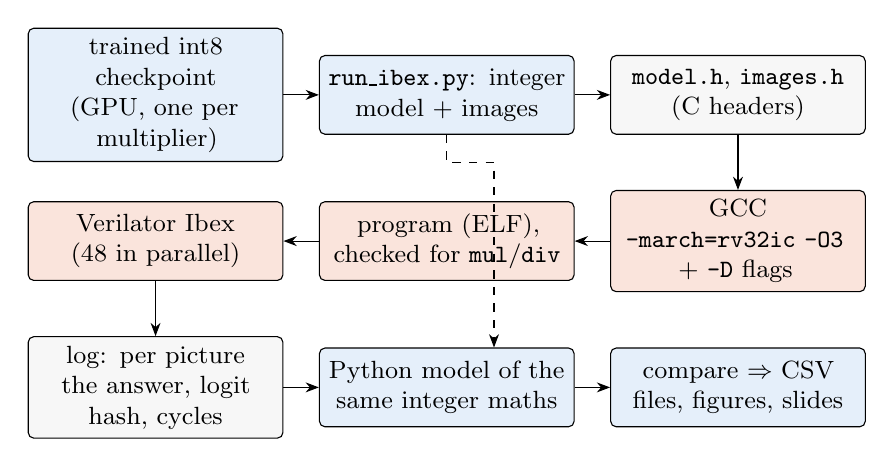
\begin{tikzpicture}[>=Stealth,font=\small,node distance=0.45cm,
  blk/.style={draw,rounded corners=2pt,align=center,minimum height=1.0cm,text width=3.0cm,fill=gray!6},
  py/.style={blk,fill=roba!12}, hw/.style={blk,fill=twoit!18}]
  \node[py] (ck) {trained int8 checkpoint\\(GPU, one per multiplier)};
  \node[py,right=of ck] (exp) {\file{run\_ibex.py}: integer model + images};
  \node[blk,right=of exp] (h) {\file{model.h}, \file{images.h}\\(C headers)};
  \node[hw,below=0.7cm of h] (gcc) {GCC \code{-march=rv32ic -O3}\\+ \code{-D} flags};
  \node[hw,left=of gcc] (elf) {program (ELF), checked for \code{mul}/\code{div}};
  \node[hw,left=of elf] (sim) {Verilator Ibex\\(48 in parallel)};
  \node[blk,below=0.7cm of sim] (log) {log: per picture the answer, logit hash, cycles};
  \node[py,right=of log] (ref) {Python model of the same integer maths};
  \node[py,right=of ref] (csv) {compare $\Rightarrow$ CSV files, figures, slides};
  \draw[->] (ck) -- (exp); \draw[->] (exp) -- (h); \draw[->] (h) -- (gcc); \draw[->] (gcc) -- (elf);
  \draw[->] (elf) -- (sim); \draw[->] (sim) -- (log); \draw[->] (log) -- (ref); \draw[->] (ref) -- (csv);
  \draw[->,dashed] (exp.south) -- ++(0,-0.35) -| ($(ref.north)+(0.6,0)$);
\end{tikzpicture}
\caption{The Phase~2 pipeline. Blue boxes run in Python on the server, orange boxes build and run the
program for the simulated chip.}
\label{fig:flow}
\end{figure}

Step by step, for one dataset, one network and one \emph{configuration} (a multiplier plus options):
\begin{enumerate}
  \item \textbf{Load the checkpoint} fine-tuned at int8 with that multiplier (the table-of-squares runs use the
        exact one).
  \item \textbf{Build the integer model} (\code{int\_model}): int8 weights, $M$ and $C$ per neuron
        (Section~\ref{sec:quant}), written as C arrays into \file{model.h}.
  \item \textbf{Quantize the first 100 test pictures} to int8 and write them, 10 per batch, into
        \file{images.h}.
  \item \textbf{Compute the expected answers in Python}: \code{ref\_forward} repeats exactly the integer
        arithmetic of the C program, bit for bit, and computes a \emph{logit hash} of the 10 scores.
  \item \textbf{Compile} \file{hw/sw/dnn.c} with flags that pick the multiplier and the method, for example
        \code{-DMULT\_NZ=roba\_dn1\_nz} (fused RoBA-Dn1) or \code{-DSQTAB} (table of squares).
  \item \textbf{Simulate}: every batch runs in its own Verilator process, 48 at a time on the server.
        The program prints one line per picture:\\
        {\footnotesize\code{IMG,<index>,<label>,<prediction>,<logit hash>,<total cycles>,<cycles per layer>}}.
  \item \textbf{Compare}: the prediction and the logit hash must equal the Python ones for every picture.
        The summaries go to \file{results/ibex/*.csv}.
\end{enumerate}

\begin{example}[: what a logit hash is for]
The 10 scores of a picture are 64-bit integers, e.g.\ $(-1043, 2210, \dots)$. Comparing all of them for
10{,}400 pictures would make long log files. Instead, the program mixes the 10 numbers into one 32-bit
fingerprint (rotate, XOR, repeat). If even one bit of one score differs, the fingerprint is completely
different. Equal hashes means equal scores.
\end{example}

\paragraph{The four stages of \file{hw/run\_ibex.py}.}
\begin{itemize}
  \item \code{--stage mult}: time one multiplication (10{,}000 of them per routine and operand size).
  \item \code{--stage dnn}: both networks, both datasets, eight multipliers fused into the loop, plus the
        table of squares: 36 configurations.
  \item \code{--stage call}: the same eight multipliers called once per product, as in the paper: 32
        configurations.
  \item \code{--stage zeroskip}: exact, Dn1 and the table, each with/without zero skipping and with
        normalised/raw pixels: 48 configurations.
\end{itemize}
In total: 116 configurations $\times$ 100 pictures = 11{,}600 simulated inferences (10{,}400 different
ones, because 12 zeroskip configurations repeat the dnn ones), about 160 billion simulated clock cycles in
roughly 70 minutes on 48 CPU cores. A finished simulation is reused only if the compiled program is
byte-for-byte the same (its SHA-256 hash matches), so a rerun after an unrelated change is quick.
\newpage

\section{Phase 2 results: the networks on Ibex}\label{sec:ibexres}

\subsection{One multiplication at a time}\label{sec:multbench}

First, the simplest measurement (\file{hw/sw/mult\_bench.c}, the paper's ``MULT kernel''): call each
routine 10{,}000 times on random unsigned numbers of 4, 8, 16 and 31 bits, and divide the cycle count by
10{,}000. This includes the call, loading the two numbers and the loop, like a real program.

\begin{figure}[H]
\centering
\includegraphics[width=\linewidth]{mult_bench}
\caption{Cycles per multiplication. Left: with the LOD instruction. Right: with LOD done in software.
The exact shift-and-add (black) grows with the size of the numbers. RoBA-Dn1 (blue, solid) stays at 28
cycles for any size, but only with the instruction: in software it costs 91--103 cycles.}
\end{figure}

\begin{table}[H]
\centering
\small
\begin{tabular}{lrrrr}
\toprule
 & \multicolumn{2}{c}{with LOD instruction} & \multicolumn{2}{c}{LOD in software}\\
\cmidrule(lr){2-3}\cmidrule(lr){4-5}
Multiplier & 8-bit & 31-bit & 8-bit & 31-bit\\
\midrule
Exact (shift-and-add) & 84.1 & 279.6 & 84.1 & 279.6\\
Mitchell & 33.5 & 34.0 & 96.5 & 109.0\\
DRUM6 & 98.5 & 101.0 & 148.8 & 164.0\\
RoBA-Dn1 & \textbf{28.0} & \textbf{28.0} & 91.0 & 103.0\\
RoBA-UpDn & 42.9 & 43.0 & 112.4 & 124.5\\
RoBA-Dn2 & 41.4 & 42.0 & 149.7 & 176.9\\
RoBA-UpDnDn & 71.5 & 72.0 & 192.7 & 219.8\\
RoBA-(UpDn)2 & 83.9 & 86.0 & 209.3 & 238.5\\
\bottomrule
\end{tabular}
\caption{Cycles per multiplication (\file{results/ibex/mult\_bench.csv}). Exact needs no LOD, so its two
columns are the same.}
\end{table}

\begin{keyidea}
With LOD, Dn1 is $84/28 = \mathbf{3.0\times}$ faster than exact for 8-bit numbers and
$280/28 = \mathbf{10\times}$ for 31-bit numbers. Without the instruction, it is \emph{slower} than exact.
The new instruction is what makes approximate multiplication worth it.
\end{keyidea}

\subsection{Whole networks, one routine call per multiplication}

Now the real thing: a whole picture through the network, written the way the paper does it. Every product
calls a small wrapper, \code{mul\_s(a, w)}, which checks for zero, takes the absolute values, calls the
multiplier routine and puts the sign back.

\begin{figure}[H]
\centering
\includegraphics[width=\linewidth]{ibex_call}
\caption{Million cycles per picture (mean of the first 100 test pictures), one routine call per
multiplication.}
\end{figure}

\begin{table}[H]
\centering
\small
\begin{tabular}{lrrrr}
\toprule
Multiplier & MNIST MLP & MNIST LeNet-5 & Fashion MLP & Fashion LeNet-5\\
\midrule
Exact & 16.89 & 29.62 & 16.04 & 29.32\\
Mitchell & 10.59 & 19.17 & 9.87 & 19.16\\
DRUM6 & 22.61 & 34.23 & 22.94 & 35.08\\
RoBA-Dn1 & \textbf{9.25} (1.83$\times$) & \textbf{17.73} (1.67$\times$) & \textbf{8.75} (1.83$\times$) & \textbf{17.59} (1.67$\times$)\\
RoBA-UpDn & 11.91 & 21.44 & 11.96 & 21.79\\
RoBA-Dn2 & 11.93 & 21.03 & 11.34 & 20.98\\
RoBA-UpDnDn & 17.36 & 28.60 & 17.95 & 29.48\\
RoBA-(UpDn)2 & 19.96 & 31.67 & 20.32 & 32.42\\
\bottomrule
\end{tabular}
\caption{Million cycles per picture, one call per product (\file{results/ibex/dnn\_call\_summary.csv}).
In brackets: how many times faster than exact.}
\end{table}

Two surprises:
\begin{enumerate}
  \item Dn1 is 3$\times$ faster per multiplication, but only \textbf{1.7--1.8$\times$} faster per picture.
  \item DRUM6, UpDnDn and (UpDn)2 are \textbf{slower than exact}. Network numbers are only 7 bits plus a sign,
        so the exact shift-and-add loop runs at most 7 rounds. That is cheap enough that methods doing
        two rounds of RoBA, or a small exact multiply, cannot beat it.
\end{enumerate}
The next subsection explains the first surprise.

\subsection{Where does the time go?}

\file{hw/profile\_ibex.py} runs one picture with Ibex's \emph{instruction tracer} switched on. It writes one
line for every instruction executed (about 1~GB of text per picture!), with the address of the instruction
and how many cycles it took. Using the program's debug information, every address is mapped back to the C
function and line it came from, and the cycles are added up per category. The traced total matches the CPU's
cycle counter within 0.1\%.

\begin{figure}[H]
\centering
\includegraphics[width=\linewidth]{profile}
\caption{Share of the time of one Fashion-MNIST picture, with one call per multiplication.}
\label{fig:profile}
\end{figure}

For the exact MLP, the multiplier routine itself takes \textbf{64\%} of the time. Another 17\% is the
sign-and-zero wrapper around it, and the rest is loading the numbers, the loop counter and adding up. For
Dn1, the routine shrinks to \textbf{35\%}, and the wrapper and loop now cost more than the multiplication.

\begin{example}[: Amdahl's law, the limit of speeding up one part]
Say a job takes 100 seconds and 64 seconds of it are multiplication. Even if multiplication became
\emph{free}, the other 36 seconds stay. The best possible speed-up is $100/36 = 2.8\times$.
In general: if a part takes a share $f$ of the time and you make it $k$ times faster, the whole job becomes
\[
  \text{speed-up} = \frac{1}{(1-f) + f/k}.
\]
For Dn1: $f = 0.64$, $k = 3$: $1/(0.36 + 0.213) = 1.74\times$. Close to the measured 1.83$\times$. The lesson:
after making the multiplier fast, the rest of the loop becomes the bottleneck.
\end{example}

\subsection{Writing the loop more cleverly: the fused MAC}\label{sec:fused}

To shrink the ``rest'', we wrote the multiply-accumulate loop differently (default build of
\file{hw/sw/dnn.c}, with the routines from \file{csrc/roba\_core.h}). We made the same three changes for
\emph{every} multiplier, exact included, so the comparison stays fair.

\paragraph{1. Inline the routine.} Instead of calling a function for every product (jump there, save
registers, jump back), the multiplier's few instructions are copied directly into the loop. The zero check
is done once per product (the old wrapper and the routine each checked).

\paragraph{2. Store weights as sign and size.} Normally $-5$ is stored as \code{11111011} (``two's
complement''), and getting its size needs a test and a negation. We store each weight as one byte with
bit~7 = the sign and bits 0--6 = the size:
\[
  +5 \to \texttt{0\,0000101} = \texttt{0x05},\qquad -5 \to \texttt{1\,0000101} = \texttt{0x85}.
\]
Then the size is one instruction (\code{byte \& 127}) and the sign another (\code{byte >> 7}). This
conversion is done once, when the program starts, outside the timed part (a real device would store the
weights like this).

\paragraph{The sign without a jump.} After multiplying the sizes, the result $r$ must be negated if the two
signs differ. A jump (``if negative, negate'') costs extra cycles on Ibex when it is taken. Instead we use a
trick: let $s = 0$ if the signs agree and $s = -1$ (all bits 1) if they differ. Then
\[
  (r \oplus s) - s = \begin{cases} r & s = 0\\ -r & s = -1\end{cases}
\]
because XOR with all ones flips every bit ($\sim r = -r-1$), and subtracting $-1$ adds 1.
\begin{example}[: the branch-free sign]
$r = 128$, $s = -1$: $128 \oplus (-1) = -129$, and $-129 - (-1) = -128$. Correct, with no jump.
With $s=0$: $128\oplus 0 - 0 = 128$.
\end{example}

\paragraph{3. After ReLU, inputs are never negative.} Every layer except the first gets its input from a
ReLU, so the input is $\ge 0$: no need to take its absolute value or look at its sign.

\begin{lstlisting}[language=C]
/* acc + a*w for an activation known to be >= 0 (after ReLU), from hw/sw/dnn.c */
static inline int32_t mac_r(int32_t acc, int32_t a, uint8_t w)
{
    uint32_t ub = w & 0x7Fu;                    /* |w|                         */
    if (a == 0 || ub == 0)                      /* one zero check              */
        return acc;
    int32_t r = (int32_t)MULT_NZ((uint32_t)a, ub);   /* e.g. roba_dn1_nz, inlined */
    int32_t s = -(int32_t)((uint32_t)w >> 7);   /* -1 if w < 0, else 0         */
    return acc + ((r ^ s) - s);                 /* add r or -r, no branch      */
}
\end{lstlisting}

\begin{figure}[H]
\centering
\includegraphics[width=\linewidth]{fused}
\caption{Fashion-MNIST: one call per multiply (white circles) against fused into the loop (filled). Every
multiplier gets faster; RoBA-Dn1 gains the most on LeNet-5.}
\end{figure}

\begin{table}[H]
\centering
\small
\begin{tabular}{lrrrr}
\toprule
Multiplier (fused) & MNIST MLP & MNIST LeNet-5 & Fashion MLP & Fashion LeNet-5\\
\midrule
Exact & 13.91 & 24.04 & 13.49 & 22.95\\
Mitchell & 8.61 (1.62$\times$) & 11.82 (2.03$\times$) & 8.14 (1.66$\times$) & 12.16 (1.89$\times$)\\
DRUM6 & 15.87 & 26.01 & 15.45 & 27.18\\
RoBA-Dn1 & \textbf{7.12 (1.95$\times$)} & \textbf{10.19 (2.36$\times$)} & \textbf{7.05 (1.91$\times$)} & \textbf{10.21 (2.25$\times$)}\\
RoBA-UpDn & 10.13 & 15.42 & 9.73 & 15.70\\
RoBA-Dn2 & 10.00 & 13.62 & 9.85 & 13.78\\
RoBA-UpDnDn & 14.94 & 22.33 & 14.42 & 23.03\\
RoBA-(UpDn)2 & 17.87 & 25.87 & 17.25 & 26.78\\
\bottomrule
\end{tabular}
\caption{Million cycles per picture with the fused loop (\file{results/ibex/dnn\_summary.csv}); in brackets
the speed-up over fused exact. Compared with the call version: exact 16.0 $\to$ 13.5 (Fashion MLP), Dn1
8.75 $\to$ 7.05, and Dn1 on Fashion LeNet-5 17.6 $\to$ 10.2 ($1.72\times$).}
\end{table}

Here is what the compiler made of the fused Dn1 loop for the MLP's first layer: 26 instructions per product,
and only 10 when the input is 0 (it jumps straight to label 2).
\begin{lstlisting}[language=asm]
      lb    a5,0(a0)      # load x
      addi  a0,a0,1
      j     1f
1:    srai  a7,a5,31      # sign of x
      xor   t3,a7,a5
      lbu   a3,0(a1)      # load w (sign-magnitude byte)
      sub   t3,t3,a7      # |x|
      beqz  a5,2f         # x = 0: skip
      andi  a5,a3,127     # |w|
      beqz  a5,2f         # w = 0: skip
      lod   a6,t3         # pa = LOD(|x|)      <- the new instruction
      lod   t1,a5         # pb = LOD(|w|)      <- the new instruction
      sll   a5,a5,a6      # |w| << pa
      srli  a4,a3,7       # sign of w
      sll   t3,t3,t1      # |x| << pb
      sll   a6,t5,a6      # 1 << pa
      neg   a4,a4
      add   a5,a5,t3
      sll   a6,a6,t1      # 2^(pa+pb)
      xor   a4,a4,a7      # combined sign s
      sub   a5,a5,a6      # Dn1 product r
      xor   a5,a5,a4      # (r ^ s)
      sub   a5,a5,a4      #   - s
      add   a2,a2,a5      # acc += product
2:    addi  a1,a1,1
      bne   a1,t0,loop
\end{lstlisting}

\subsection{No multiplier at all: a table of squares}\label{sec:sqtab}

There is an old trick (it was used by people multiplying with tables of squares before calculators). Since
$(x+w)^2 = x^2 + 2xw + w^2$,
\[
  x\cdot w = \frac{(x+w)^2 - x^2 - w^2}{2}.
\]
A square can be \emph{looked up} in a table instead of computed. So a product becomes three lookups, two
subtractions and a halving. This is called the \textbf{polarization identity}.

\begin{example}[: products from squares]
$3\times5$: $\big((3+5)^2 - 3^2 - 5^2\big)/2 = (64 - 9 - 25)/2 = 30/2 = 15$.\\
$3\times(-5)$: $\big((-2)^2 - 9 - 25\big)/2 = (4-34)/2 = -15$. Negative numbers just work.
\end{example}

It gets much better for a whole neuron. Add up the identity over all inputs:
\[
  \sum_k x_k w_k = \frac{1}{2}\Big(\underbrace{\sum_k S(x_k+w_k)}_{\text{1 lookup per MAC}}
  - \underbrace{\sum_k S(x_k)}_{\text{same for every neuron}}
  - \underbrace{\sum_k S(w_k)}_{\text{fixed: computed in advance}}\Big),\qquad S(v) = v^2.
\]
\begin{itemize}
  \item $\sum S(w_k)$ depends only on the weights, so it is computed once, before running (outside the
        timed part, like the weights themselves).
  \item $\sum S(x_k)$ depends only on the layer's input, which is the \emph{same} for all 256 neurons of the
        MLP's first layer. It is computed once and shared.
  \item So each MAC costs about \textbf{one table lookup and one addition}.
\end{itemize}

\begin{example}[: a two-input neuron]
$x = (3, 2)$, $w = (5, -1)$. Exact: $15 - 2 = 13$.
$\sum S(x+w) = S(8) + S(1) = 64 + 1 = 65$; $\sum S(x) = 9 + 4 = 13$; $\sum S(w) = 25 + 1 = 26$.
$(65 - 13 - 26)/2 = 26/2 = 13$. Exact, with no multiplication. (The number before halving is always
even, because it equals $2\sum x_kw_k$, so the halving is exact.)
\end{example}

\paragraph{The table.} Inputs and weights are int8 ($-127\dots127$), so $x+w$ is in $-254\dots254$: 509
entries. The largest square, $254^2 = 64{,}516$, fits in 16 bits, so the table is $509\times 2 =
1{,}018$ bytes, about \textbf{1~KB}. It is built at start-up without any multiplication, using
$(n+1)^2 = n^2 + 2n + 1$: start at 0 and add $1, 3, 5, 7, \dots$ $\to 0, 1, 4, 9, 16, \dots$

\paragraph{Convolutions.} In a convolution each output position sees a different $5\times5$ window of
the input, so $\sum S(x)$ is different per position, but it is still the same for all filters at that
position. The program computes all window sums once per layer with ``box sums'' (add 5 neighbours across,
then 5 down) and shares them across the 6 (or 16) filters.

The inner loop is now 10 instructions instead of 26, and none of them is LOD:
\begin{lstlisting}[language=asm]
      lb    a5,0(a4)      # load x
      lb    a0,0(a3)      # load w
      addi  a4,a4,1
      addi  a3,a3,1
      add   a5,a5,a0      # x + w
      slli  a5,a5,1       # times 2 bytes per entry
      add   a5,a5,a1      # address in the table
      lhu   a5,0(a5)      # S[x + w]
      add   a2,a2,a5      # d += S[x + w]
      bne   s1,a4,loop
\end{lstlisting}

\begin{figure}[H]
\centering
\includegraphics[width=\linewidth]{sqtab}
\caption{Million cycles per picture and speed-up over fused exact. The table of squares is the fastest
everywhere, and its products are exact.}
\end{figure}

\begin{figure}[H]
\centering
\includegraphics[width=\linewidth]{layers}
\caption{Cycles per layer (Fashion-MNIST). In the MLP almost everything is the first layer
($784\to256$, 85\% of the multiplications). In LeNet-5, conv2 is the largest part.}
\end{figure}

\begin{table}[H]
\centering
\small
\begin{tabular}{lrrrr}
\toprule
 & MNIST MLP & MNIST LeNet-5 & Fashion MLP & Fashion LeNet-5\\
\midrule
Exact, fused & 13.91 & 24.04 & 13.49 & 22.95\\
RoBA-Dn1, fused & 7.12 (1.95$\times$) & 10.19 (2.36$\times$) & 7.05 (1.91$\times$) & 10.21 (2.25$\times$)\\
Square table & \textbf{3.87 (3.59$\times$)} & \textbf{7.58 (3.17$\times$)} & \textbf{3.87 (3.49$\times$)} & \textbf{7.57 (3.03$\times$)}\\
\bottomrule
\end{tabular}
\caption{Million cycles per picture. The table is 1.3--1.8$\times$ faster than fused Dn1, with exact
products and no LOD.}
\end{table}

\begin{kid}
Notice that the table method takes \emph{exactly} the same time (3.87 million cycles) for an MNIST
digit and a Fashion-MNIST shoe. It does the same lookups no matter what the numbers are. The RoBA and
exact loops skip zeros and their speed depends on the numbers, so their times differ a little between
datasets.
\end{kid}

\begin{careful}
The table trick depends on two things that are true here but not everywhere. (1) Ibex's memory answers in
one cycle; with slow flash memory or a cache, every lookup could cost more. (2) The numbers are 8-bit. For
16-bit numbers the table would need about 131{,}000 entries of 4 bytes each, roughly \textbf{512~KB}, too
big for a small chip, while the LOD-based RoBA routines cost the same for any size.
\end{careful}

\paragraph{A tempting idea that does not work: approximate squares.} One could replace the table with
RoBA-style \emph{approximate} squares, $\tilde S(x) = (|x| \ll (k+1)) - (1\ll 2k)$ with $k = \text{LOD}(|x|)$.
This is a straight-line estimate of $x^2$ that is always a little too small. The problem is that the
three squares are big numbers, and the product is the small difference between them, so small errors in
the squares become large errors in the product:
\begin{example}[: why approximate squares fail]
$3\times4 = 12$. $\tilde S(7) = (7\ll3) - (1\ll4) = 56-16 = 40$ (true 49); $\tilde S(3) = 12-4 = 8$
(true 9); $\tilde S(4) = 16$ (exact, a power of two).
$(40 - 8 - 16)/2 = 8$ instead of 12: \textbf{33\% too small}, although no square was more than 18\% off.
\end{example}
We tested it on the GPU: the networks lost 6--15 accuracy points in 3 of the 4 cases, so it was rejected.
The exact table is both exact and fastest.

\subsection{Skipping zeros, and feeding raw pixels}\label{sec:zeroskip}

Anything times zero is zero, so a zero input could be skipped entirely. How many zeros are there?
\begin{itemize}
  \item In \textbf{hidden layers}, many: ReLU turns every negative value into 0.
  \item In the \textbf{input picture}, none! Remember that normalising turns black into $-0.424$ (MNIST),
        not 0. Most of an MNIST picture is black background, all of it non-zero.
\end{itemize}

\paragraph{Raw pixels: folding the normalisation into the first layer.} The first layer computes
$\sum_k w_k\,\frac{p_k - \text{mean}}{\text{std}} + b$. This can be rewritten as
\[
  \sum_k \underbrace{\frac{w_k}{\text{std}}}_{\text{new weight}}\, p_k
  \;+\; \underbrace{\Big(b - \text{mean}\sum_k \frac{w_k}{\text{std}}\Big)}_{\text{new bias}}.
\]
Same result, but now the network reads the raw pixel $p_k$, and black is exactly 0.
\begin{example}[: folding one weight]
MNIST, $w = 0.6$, pixel $p = 0.5$. Original: $0.6\times(0.5-0.1307)/0.3081 = 0.6\times1.1986 = 0.719$.
Folded: new weight $0.6/0.3081 = 1.947$, bias change $-0.1307\times1.947 = -0.254$;
$1.947\times0.5 - 0.254 = 0.719$. The same.
\end{example}
The raw int8 input is $\text{round}(127\,p)$, computed from the original 8-bit pixel $k$ as
$(254k + 255)\,\text{div}\,510 = \text{round}(127k/255)$. After this, \textbf{81\% of MNIST pixels and 51\%
of Fashion-MNIST pixels are exactly 0}.

\begin{careful}
For LeNet-5 there is a detail at the border. conv1 pads the picture with zeros so that the output is still
$28\times28$. With normalised inputs, a padded 0 means ``an average pixel''; with raw inputs it means
``black''. So the new bias depends on how many of the filter's 25 taps fall on the real picture, and conv1
gets one bias per output position (a $6\times28\times28$ map) instead of one per filter
(\code{C0\_PER\_POSITION} in the code).
\end{careful}

\paragraph{Skipping (``+zs'').} The multiplier loops already skip zero products one at a time (the zero
check). With \code{ZERO\_SKIP}, a fully connected layer first collects the non-zero inputs and their positions
once, and then every neuron loops only over those. For the table method skipping needs more work per
remaining term: a zero input adds $S(0+w) - S(0) - S(w) = 0$, so it can be dropped, but then the precomputed
$\sum S(w)$ no longer matches, and the loop must use $S(x+w) - S(w)$: \emph{two} lookups per term.

\begin{figure}[H]
\centering
\includegraphics[width=\linewidth]{zeroskip}
\caption{The ablation: each method with normalised or raw pixels, with or without skipping. The labels give
the speed-up over exact with normalised input (the first bar).}
\end{figure}

\begin{table}[H]
\centering
\small
\begin{tabular}{llrrrr}
\toprule
Method & Setting & MNIST MLP & MNIST LeNet-5 & Fashion MLP & Fashion LeNet-5\\
\midrule
\multirow{4}{*}{Exact} & normalised & 13.91 & 24.04 & 13.49 & 22.95\\
 & + skip & 13.49 & 23.85 & 13.96 & 22.76\\
 & raw & 5.45 & 17.81 & 7.75 & 19.73\\
 & raw + skip & 3.18 & 17.64 & 6.82 & 19.60\\
\midrule
\multirow{4}{*}{RoBA-Dn1} & normalised & 7.12 & 10.19 & 7.05 & 10.21\\
 & + skip & 6.92 & 9.94 & 7.00 & 10.16\\
 & raw & 3.57 & 8.86 & 4.30 & 9.68\\
 & raw + skip & 1.58 & 8.69 & 3.23 & 9.62\\
\midrule
\multirow{4}{*}{Square table} & normalised & 3.87 & 7.58 & 3.87 & 7.57\\
 & + skip & 5.10 & 8.20 & 4.99 & 8.31\\
 & raw & 3.87 & 7.57 & 3.64 & 7.62\\
 & raw + skip & \textbf{1.33} & \textbf{7.38} & \textbf{2.70} & 7.93\\
\bottomrule
\end{tabular}
\caption{Million cycles per picture (\file{results/ibex/zeroskip\_summary.csv}). Best per column in bold
(Fashion LeNet-5: the table with raw pixels and no skip, 7.62, is about as fast as the normalised table).}
\end{table}

What this shows:
\begin{itemize}
  \item \textbf{Raw pixels are the big win.} Exact on the MNIST MLP drops from 13.9 to 5.5 million cycles just
        by giving the existing zero check something to skip.
  \item \textbf{The best MLP result:} table + raw + skip on MNIST, \textbf{1.33 million cycles, $10.5\times$ faster}
        than exact with normalised input. On Fashion (fewer black pixels) it is $5.0\times$.
  \item \textbf{Skipping without raw pixels does not help}, and it makes the table \emph{slower}
        ($3.87\to4.99$ on Fashion), because each remaining term now needs two lookups.
  \item \textbf{LeNet-5 hardly changes}: most of its work is conv2, whose input comes after ReLU and pooling
        and is not affected by the raw pixels, and the convolution can only skip tap by tap.
\end{itemize}

\begin{table}[H]
\centering
\small
\begin{tabular}{lcccc}
\toprule
 & \multicolumn{2}{c}{MNIST MLP} & \multicolumn{2}{c}{Fashion MLP}\\
\cmidrule(lr){2-3}\cmidrule(lr){4-5}
 & normalised & raw & normalised & raw\\
\midrule
Exact / table & 98.41 & 98.46 & 89.75 & 89.69\\
RoBA-Dn1 & 98.36 & 98.42 & 89.53 & 89.53\\
\bottomrule
\end{tabular}
\caption{Accuracy on all 10{,}000 test pictures (from the bit-exact Python model) with normalised and raw
input: raw pixels cost no accuracy. Skipping never changes a result. (LeNet-5: MNIST 99.18/99.19, Fashion
90.83/90.80 for exact.)}
\end{table}

\subsection{Energy}\label{sec:energy}

Energy is power multiplied by time: $E = P\times T$. Time is proportional to cycles. For power we use the
paper's synthesis results, relative to a core with a single-cycle hardware multiplier ($P = 1$):
\begin{itemize}
  \item Multiplierless core \emph{with} LOD: 17.1\% less power, so $P_{\text{LOD}} = 1 - 0.171 = 0.829$.
  \item LOD itself adds 4.5\%, so the multiplierless core \emph{without} LOD has
        $P_{\text{none}} = 0.829/1.045 = 0.793$.
\end{itemize}
Exact and the table of squares do not use LOD, so they run on the cheaper 0.793 core. Mitchell, DRUM6 and all
RoBA methods need the LOD core (0.829).

\begin{example}[: energy of one Fashion-MNIST MLP picture (fused)]
\begin{tabular}{@{}lrl@{}}
Exact: & $13.49 \times 0.793 = 10.70$ & (reference, 1.00)\\
RoBA-Dn1: & $7.05 \times 0.829 = 5.84$ & $\Rightarrow 5.84/10.70 = \mathbf{0.55}$\\
Square table: & $3.87 \times 0.793 = 3.07$ & $\Rightarrow \mathbf{0.29}$\\
RoBA-(UpDn)2: & $17.25\times0.829 = 14.30$ & $\Rightarrow 1.34$ (more energy than exact!)
\end{tabular}
\end{example}

\begin{figure}[H]
\centering
\includegraphics[width=\linewidth]{energy}
\caption{Energy per picture relative to exact (fused, Fashion-MNIST). Below the dashed line saves energy.}
\end{figure}

\begin{keyidea}
Because LOD raises the power by 4.5\%, an approximate method has to be at least 4.5\% faster than exact
just to break even. Dn1 is about 2$\times$ faster, so it needs only \textbf{0.44--0.55} of the energy.
The two-step methods and DRUM6 are slower than exact and \emph{waste} energy. The table of squares needs
\textbf{0.28--0.33}.
\end{keyidea}

\begin{careful}
These energies are \emph{estimates}: measured cycles times the paper's relative power numbers. The real
power also depends on what the program does (memory accesses use more than additions, for example). A
real power measurement needs the FPGA or a chip.
\end{careful}

\subsection{How do we know the simulated chip computed the right thing?}

\begin{itemize}
  \item \textbf{All 10{,}400 different inferences} (100 pictures $\times$ 104 distinct configurations) gave
        \textbf{exactly the same scores, bit for bit,} as the Python model of the same integer arithmetic
        (\code{logits\_match\_ref = 1.0} in every row of the CSV files).
  \item The 32 ``call'' configurations were run in two separate runs, from rebuilt programs, and gave
        identical cycle counts and answers.
  \item Ibex accuracy on these 100 pictures: MNIST 100\% for every configuration; Fashion 90--91\% (MLP)
        and 85--88\% (LeNet-5). With 100 pictures one picture is one point, so these numbers move more than
        the full-test numbers. The full-test accuracy comes from the bit-exact Python model.
  \item The integer Ibex model agrees with the GPU's int8 model on 97--100\% of the 100 pictures. The small
        difference is not an error: the GPU version rescales with decimal arithmetic, the integer version with
        $M$ and a shift, so a value right at a rounding edge (like 6.5) can round the other way and, rarely,
        flip an answer. Over the full test set the two agree within 0.05 points for exact and within about
        0.3 points for RoBA-Dn1 (Fashion LeNet-5: 90.49\% integer vs 90.77\% GPU).
\end{itemize}
\newpage

\section{Putting it all together}\label{sec:wrap}

\subsection{The story of the numbers}

Follow one Fashion-MNIST MLP picture through the whole project:

\begin{center}
\small
\begin{tabular}{lrrl}
\toprule
Version & million cycles & vs.\ start & what changed\\
\midrule
Exact, one call per multiply (paper style) & 16.04 & 1.00$\times$ & starting point\\
RoBA-Dn1, one call per multiply & 8.75 & 1.83$\times$ & LOD + approximate multiply\\
Exact, fused loop & 13.49 & 1.19$\times$ & better loop, exact multiply\\
RoBA-Dn1, fused loop & 7.05 & 2.28$\times$ & better loop + RoBA\\
Table of squares & 3.87 & 4.14$\times$ & no multiply at all, exact\\
Table of squares, raw pixels + skip & 2.70 & 5.94$\times$ & also skip the black background\\
\bottomrule
\end{tabular}
\end{center}

And the accuracy of all of them on the full test set stays between 89.5\% and 89.8\%.

\subsection{What we learned}

\begin{enumerate}
  \item \textbf{Approximate multiplication does not hurt these networks.} Every one of the seven
        approximate multipliers stays within 0.75 points of exact at int8, most within 0.2 points, even
        RoBA-Dn1, which is 9\% too small on average. Fine-tuning recovers most of the rest.
  \item \textbf{The LOD instruction is essential.} With it, Dn1 costs 28 cycles per multiply at any size;
        without it, 91 or more, which is slower than exact.
  \item \textbf{Faster multiplies expose the rest of the loop.} Per multiply Dn1 is 3$\times$ faster, per
        picture only 1.8$\times$, because the wrapper and the loop then dominate (Amdahl's law). Fusing the
        multiply into the loop raises Dn1's advantage to 1.9--2.4$\times$.
  \item \textbf{More accurate is not always better on this CPU.} The two-step RoBA methods and DRUM6 are
        slower than exact for 8-bit numbers and use more energy. Only the one-step methods (Dn1, UpDn,
        Mitchell) and Dn2 pay off.
  \item \textbf{For int8, an exact table of squares wins.} It needs 1~KB and no new instruction, gives exact
        products, and is 3.0--3.6$\times$ faster than exact (1.3--1.8$\times$ faster than Dn1).
  \item \textbf{Zeros matter.} Feeding raw pixels (so the background is 0) and skipping zeros brings the MNIST
        MLP to 10.5$\times$.
  \item \textbf{Energy follows cycles.} LOD adds 4.5\% power, so Dn1 at about 2$\times$ the speed uses roughly
        half the energy, and the table about 0.3.
  \item \textbf{It holds on real tasks, and precision picks the winner} (Phase 3). On CIFAR-10, keyword spotting
        and machine-sound anomaly detection, with three seeds: at int8 the table wins (2.0--2.6$\times$, exact);
        at int16 the table does not fit and RoBA wins (Dn1 2.9--3.3$\times$ at a third of the energy, Dn2
        2.4--2.5$\times$ within 0.2 points of exact); at int4 nothing gains much.
  \item \textbf{It holds on a real chip, and memory speed matters} (Phase 4). On the Zybo FPGA the Ibex gives the
        same outputs as the Python model (960/960) and, from on-chip RAM, exactly the simulated cycles (240/240).
        The LOD costs no measurable area. With data in DDR (about 15 cycles per access) the table drops to about
        exact speed, while RoBA-Dn1 keeps 1.3--1.4$\times$ at int8 and 2.0--2.2$\times$ at int16.
\end{enumerate}

\subsection{Limits: what these results do not show}

\begin{itemize}
  \item \textbf{One training seed} per dataset in Phases 1--2 (Phase 3 uses three): there, accuracy differences
        below about 0.1 points are noise.
  \item \textbf{100 test pictures} on Ibex per configuration (the full 10{,}000 are covered by the bit-exact
        Python model). The cycle counts vary very little from picture to picture, so 100 is enough for them.
  \item \textbf{Energy is estimated}, not measured: cycles times relative power from the paper. The FPGA's
        Vivado power report is itself an estimate (default switching rates, 1~mW resolution); no current was
        measured on the board.
  \item \textbf{One-cycle memory} in the simulator. The FPGA (Phase 4) measured the other extreme, DDR at about
        15 cycles per access; caches or flash wait states would lie in between.
  \item \textbf{Phase 3 cycles use seed 0 and 20 inputs} per configuration; accuracy uses all seeds and the
        full test sets through the bit-exact Python model.
  \item \textbf{Keyword spotting at int4 is unsolved} (about 61\% for every method); keeping the first layer at
        8 bits is the likely fix and has not been tried.
  \item \textbf{We did not measure a core with a hardware multiplier}; it would need fewer cycles, at more area
        and power.
  \item Our \textbf{Mitchell} is the classic one with the carry; the paper's Mitchell gives the same products as
        RoBA-Dn1.
\end{itemize}

\subsection{What comes next}
\begin{enumerate}
  \item The two remaining datasets in the Phase 3 pipeline: Visual Wake Words (MLPerf Tiny's person detection)
        and MNIST / Fashion-MNIST with three seeds.
  \item Fix int4 keyword spotting (first layer at 8 bits).
  \item Choosing the multiplier per layer: cheap where the network tolerates errors, accurate where it is
        sensitive.
  \item Replace the equal-power assumption by power per method: Vivado power analysis with each program's
        simulated switching activity, or a current measurement on the board.
  \item A small data cache or tighter memory layout, so that more programs run from on-chip RAM.
\end{enumerate}

\subsection{Glossary}

\begin{description}[style=nextline,leftmargin=1.2cm,font=\normalfont\bfseries]
  \item[Accumulator (\code{acc})] The running sum inside a neuron while its products are added up.
  \item[Activation] A value flowing between layers (the input of a neuron).
  \item[ALU] Arithmetic logic unit: the part of the CPU that adds, shifts, compares, and now also does LOD.
  \item[Amdahl's law] Speeding up one part of a job by $k$ only helps in proportion to that part's share of
        the time.
  \item[Approximate square] $\tilde S(v) = (2v - 2^k)\,2^k$ with $k = \mathrm{LOD}(v)$; a cheap but inexact
        square. Fails inside the polarization identity.
  \item[Approximate multiplier] A method that computes a product that is close to, but not always exactly,
        the true product, in exchange for speed or energy.
  \item[AUC] Area under the ROC curve: the chance that a random broken example scores higher than a random
        normal one. 50\% is coin tossing, 100\% is perfect.
  \item[Autoencoder] A network that squeezes its input through a narrow middle and rebuilds it; a bad rebuild
        means an unusual input.
  \item[Bare metal] A program that runs directly on the CPU, with no operating system.
  \item[Bitstream] The file that configures an FPGA into a particular circuit.
  \item[Bias] The extra number a neuron adds after its sum of products.
  \item[Block RAM] Memory blocks inside the FPGA (4~KB each, 60 on the XC7Z010); one-cycle access.
  \item[Bit, binary] A 0/1 digit; numbers written with place values 1, 2, 4, 8, \dots
  \item[Calibration] Choosing the scale that maps each layer's decimal values onto the integer range.
  \item[Checkpoint] A saved file with all the weights of a trained network.
  \item[Clock cycle] One tick of the CPU's clock; the unit we measure speed in.
  \item[Convolution] A layer that slides a small filter of weights over a picture.
  \item[Custom-0] An opcode RISC-V reserves for non-standard instructions; LOD lives there.
  \item[Cycle-accurate simulation] A simulation that reproduces the chip tick by tick, so its cycle counts
        are exact.
  \item[Depthwise-separable convolution] A $3\times3$ convolution per channel followed by a $1\times1$
        convolution across channels; about 8 times fewer multiplications. Used by DS-CNN.
  \item[DDR] The board's main memory chip: large (512~MB) but slow for the Ibex (about 15 cycles per access).
  \item[Decoder] The part of the CPU that works out what an instruction means.
  \item[DRUM6] An approximate multiplier that keeps the top 6 bits of each number and multiplies those
        exactly.
  \item[Epoch] One pass over all training pictures.
  \item[Fine-tuning] A few more training epochs, here with the approximate multiplier switched on.
  \item[Fixed point] Representing a decimal as an integer with an agreed scale (here $2^{24}$).
  \item[FPGA] A chip whose circuit can be reprogrammed; used to try out CPU designs for real.
  \item[FPGA board, Zybo] Digilent's board with a Zynq XC7Z010 (ARM processor + FPGA) used in Phase 4.
  \item[Fused MAC] Writing the multiplier directly inside the multiply-accumulate loop instead of calling it.
  \item[Ibex] A small open-source RISC-V CPU from lowRISC.
  \item[int4 / int8 / int16] Whole numbers stored in 4, 8 or 16 bits ($\pm7$, $\pm127$ or $\pm32767$ for weights).
  \item[LeNet-5] A small convolutional network: two convolution layers and three fully connected layers.
  \item[LOD] Leading-one detector: the instruction that returns the position of a number's highest 1 bit.
  \item[Logit / score] A raw output value of the last layer; the largest one is the answer.
  \item[Logit hash] A 32-bit fingerprint of the 10 scores, used to check them quickly.
  \item[Loss] A number that measures how wrong the network is; training makes it small.
  \item[M extension] The optional RISC-V instructions for multiplication and division; our core does not have
        them.
  \item[MFCC] Mel-frequency cepstral coefficients: a small ``picture of a sound'' (energy at different pitches
        over time).
  \item[MLPerf Tiny] The standard benchmark of tasks and reference networks for machine learning on tiny chips.
  \item[LUT] Look-up table: the FPGA's basic logic block; area is counted in LUTs and flip-flops.
  \item[MAC] Multiply-accumulate: one product added to a running sum.
  \item[Mitchell] A classic approximate multiplier based on logarithms.
  \item[MLP] Multi-layer perceptron: a network of fully connected layers.
  \item[MNIST, Fashion-MNIST] Datasets of $28\times28$ grey pictures: hand-written digits and clothes.
  \item[Normalisation] Shifting and scaling the pixels to be centred around 0 ($(x-\text{mean})/\text{std}$).
  \item[Polarization identity] $xw = ((x+w)^2 - x^2 - w^2)/2$: a product from three squares.
  \item[Priority encoder] A circuit that outputs the position of the highest 1 among its inputs.
  \item[QAT] Quantization-aware training: fine-tuning with the integer rounding (and here the approximate
        multiplier) switched on in the forward pass.
  \item[Quantization] Turning decimal numbers into integers with a scale.
  \item[Raw pixels] Feeding the picture without normalisation (the normalisation is folded into the first
        layer), so black is 0.
  \item[ReLU] The rule ``negative $\to$ 0, positive stays''.
  \item[ResNet] A network with shortcuts that add a block's input to its output.
  \item[Register] One of the CPU's 32 small storage slots for numbers.
  \item[RISC-V] An open instruction set; RV32I is its basic 32-bit integer version, C adds short
        instructions.
  \item[RoBA] Rounding-based approximate multiplication: round to powers of two, keep the cheap parts.
        Dn = round down, UpDn = round to the nearest, the ``2'' versions repeat it on the leftover.
  \item[Seed] The starting number of the random-number generator; a different seed gives a different
        training run.
  \item[Shift] Moving all bits left (multiply by 2) or right (divide by 2).
  \item[Shift-and-add] The exact way to multiply without a multiplier: add shifted copies.
  \item[Sign-magnitude] Storing a number as a sign bit plus its size.
  \item[Square table] A 509-entry table of $v^2$ used by the polarization identity.
  \item[Straight-through estimator] Training trick: use the approximate result going forward, pretend it
        was exact going backward.
  \item[Test accuracy] Share of unseen test pictures the network gets right.
  \item[Verilator] A tool that turns a hardware description into a fast C++ cycle-accurate simulator.
  \item[Vivado, Vitis] Xilinx tools: hardware to bitstream (with area/timing/power reports); ARM software.
  \item[WNS] Worst negative slack: the timing margin of the slowest path; positive means the clock is safe.
  \item[Zero skipping] Not doing the work for inputs that are 0.
\end{description}
\newpage

\appendix
\section{A tour of the code, file by file}\label{app:code}

\begin{figure}[H]
\centering
\footnotesize
\begin{tabularx}{\linewidth}{@{}>{\raggedright\arraybackslash}p{7.6cm}X@{}}
\toprule
\textbf{Phase 1 (GPU, Python)} & \\
\file{roba/multipliers.py} & the eight multipliers in PyTorch, as per-number ``pieces''\\
\file{roba/reference.py} & the same eight with plain Python bit operations (independent check)\\
\file{roba/matmul.py} & approximate matrix multiply and convolution from a few exact ones\\
\file{roba/nn.py} & layers with switchable multiplier and number format; MLP, LeNet-5; calibration\\
\file{roba/data.py} & reads MNIST / Fashion-MNIST and normalises the pixels\\
\file{roba/cost.py} & the early cycle and energy \emph{estimate} (replaced by Ibex measurements)\\
\file{experiments/run.py} & stages errors, train, eval, finetune $\to$ \file{results/<dataset>/}\\
\midrule
\textbf{Shared C library} & \\
\file{csrc/roba.c}, \file{roba.h} & the multipliers in C, one function each (used by the ``call'' builds)\\
\file{csrc/roba\_core.h} & the same routines as inline functions, for the fused loop\\
\file{csrc/roba\_core\_test.c} & lets the Python tests call the inline routines\\
\midrule
\textbf{Phase 2 (Ibex)} & \\
\file{hw/setup.sh}, \file{build\_sim.sh}, \file{run\_sim.sh} & install tools, build the simulator, run a program\\
\file{hw/patches/0001-ibex-lod-instruction.patch} & the LOD instruction (Section~\ref{sec:lodpatch})\\
\file{hw/sw/lod\_test.c} & checks LOD against a software loop\\
\file{hw/sw/mult\_bench.c} & cycles per multiplication\\
\file{hw/sw/dnn.c} & the integer networks for the chip, every method\\
\file{hw/sw/util.h}, \file{link\_1mb.ld}, \file{Makefile} & printing, cycle counter, memory map, builds\\
\file{hw/run\_ibex.py} & the whole Phase 2 pipeline (Figure~\ref{fig:flow})\\
\file{hw/profile\_ibex.py} & where the cycles go (instruction trace of one picture)\\
\midrule
\textbf{Phase 3 (MLPerf Tiny)} & \\
\file{tiny/data.py} & CIFAR-10, Speech Commands (MFCC) and ToyADMOS (log-mel slices), with augmentation\\
\file{tiny/models.py} & ResNet-8, DS-CNN and the autoencoder, each with a layer list (\code{spec()})\\
\file{tiny/qnet.py} & int4/8/16 quantization, QAT model, export of the integer program, bit-exact reference\\
\file{tiny/run.py} & stages train, qat, eval for 3 seeds $\to$ \file{results/tiny/<dataset>/}\\
\file{hw/sw/tiny.c}, \file{tiny\_kernels.h} & the generic integer network for Ibex: convolution, shortcuts, pooling\\
\file{hw/run\_tiny.py} & writes \file{net.h} from the program, builds, simulates, checks every output\\
\file{tests/test\_tiny.py} & 33 tests of the integer layers, the square identity and input quantization\\
\midrule
\textbf{Checks and presentation} & \\
\file{tests/test\_multipliers.py} & 35 tests: PyTorch = Python = C for every multiplier\\
\file{experiments/build\_site.py}, \file{site/template.html} & build the slide deck \file{index.html}\\
\file{doc/make\_figures.py}, \file{doc/roba\_explained.tex} & this document\\
\bottomrule
\end{tabularx}
\caption{What each file does.}
\end{figure}

\subsection{\file{roba/multipliers.py}: one description for every RoBA variant}

Each RoBA variant is just a list of rounding rules, one per step:
\begin{lstlisting}[language=Python]
ROBA_ITERATIONS = {
    "roba_dn1":    [round_dn],
    "roba_updn":   [round_updn],
    "roba_dn2":    [round_dn, round_dn],
    "roba_updndn": [round_updn, round_dn],
    "roba_updn2":  [round_updn, round_updn],
}
\end{lstlisting}
\code{factors(x, mult, side)} turns a number into its pieces (Section~\ref{sec:factors}): for each step it
rounds the current leftover \code{r}, emits \code{[rr, r - rr]} for the left number or \code{[r, rr]} for the
right number, and continues with the leftover \code{r - rr}. Summing the products of matching pieces gives the
approximate product. \code{round\_dn} and \code{round\_updn} use \code{torch.frexp}, which splits a number into
$m\times2^e$; that is the GPU's way of finding the leading one.

\subsection{\file{roba/nn.py}: switchable layers}

\code{ALinear} and \code{AConv2d} behave like PyTorch's layers but have two settings:
\code{domain} (\code{None} = normal float32, \code{"float"}, \code{"trunc"}, \code{8}, \code{16}) and
\code{mult} (one of the eight). In \code{\_forward}, for int8 it quantizes inputs and weights
(\code{fake\_quant}), computes the exact product (which carries the gradient) and the approximate one
(computed without gradient), and returns \code{ref + (acc - ref).detach()}: the value of the approximate
result with the gradient of the exact one, the straight-through estimator. \code{calibrate()} records the
largest input of every layer on 5{,}000 training pictures, which sets the activation scales.

\subsection{\file{experiments/run.py}: the GPU stages}

\begin{lstlisting}[language=bash]
python3 experiments/run.py --dataset mnist   --stage all                              # ~7 min
python3 experiments/run.py --dataset fashion --stage all --epochs 30 --ft-epochs 5    # ~10 min
\end{lstlisting}
It writes \file{results/<dataset>/eval\_<model>.csv} (one row per number format and multiplier: accuracy,
loss, agreement with exact) and \file{finetune\_<model>.csv} (accuracy before and after fine-tuning), and saves
every checkpoint in \file{checkpoints/<dataset>/} (e.g.\ \file{mlp\_ft\_int8\_roba\_dn1.pt}), which Phase~2
reads.

\subsection{\file{hw/sw/dnn.c}: one program, many methods}

The same C file is compiled differently for each configuration. The \code{-D} flags pick the method:

\begin{table}[H]
\centering
\small
\begin{tabularx}{\linewidth}{lX}
\toprule
Flags & What the multiply-accumulate does\\
\midrule
\code{-DMULT\_NZ=roba\_dn1\_nz} & fused (default): \code{mac\_g}/\code{mac\_r} with the routine inlined from
\file{roba\_core.h}, sign-magnitude weight bytes (\code{WS0}, \dots, built in \code{tables\_init})\\
\code{-DMAC\_CALL -DMULT\_U=roba\_dn1\_u} & paper style: \code{mul\_s()} calls the routine in \file{roba.c} once per
product\\
\code{-DSQTAB} & table of squares: \code{STAB[509]} built in \code{tables\_init}, $\sum S(w)$ per neuron in
\code{model\_init}, $\sum S(x)$ per layer input\\
\code{-DZERO\_SKIP} & (with any of the above) gather the non-zero inputs (\code{gather\_nz}), or skip zero taps in
convolutions\\
\code{INPUT\_NONNEG} (in \file{model.h}) & raw pixels: the first layer also uses the ``input $\ge 0$'' MAC\\
\code{C0\_PER\_POSITION} (in \file{model.h}) & LeNet-5 with raw pixels: conv1 bias per output position\\
\bottomrule
\end{tabularx}
\caption{Build options of \file{hw/sw/dnn.c}.}
\end{table}

The network itself is written once, with a macro for a fully connected layer:
\begin{lstlisting}[language=C]
static void forward(const int8_t *x, uint32_t *lc)       /* the MLP */
{
    uint32_t t = (uint32_t)cycles(), u;
    FC(x, 784, 0, 256, h1, 0, MAC_IN);                   /* layer 0: 784 -> 256 */
    u = (uint32_t)cycles(); lc[0] = u - t; t = u;        /* cycles of layer 0   */
    FC(h1, 256, 1, 128, h2, 0, MAC_R);                   /* layer 1: 256 -> 128 */
    u = (uint32_t)cycles(); lc[1] = u - t; t = u;
    FC(h2, 128, 2, 10, z, 1, MAC_R);                     /* layer 2: 128 -> 10, keep logits */
    u = (uint32_t)cycles(); lc[2] = u - t;
}
\end{lstlisting}
\code{FC} expands to the right loop for the chosen method (plain, zero-skipping, table, or table with
skipping), followed by \code{rescale()} and \code{relu\_q()} for every output. \code{main()} builds the tables,
switches on the cycle counter, runs \code{forward} on every picture in \file{images.h}, and prints the
\code{IMG,\dots} line.

\subsection{\file{hw/run\_ibex.py}: the pipeline}

\begin{itemize}
  \item \code{int\_model()}: checkpoint $\to$ int8 weights, $M$, $C$ (and the raw-pixel fold).
  \item \code{quantize\_images()}: pictures $\to$ int8 (normalised or raw).
  \item \code{ref\_forward()}: the bit-exact Python copy of \file{dnn.c}; \code{logit\_hash()} the same
        fingerprint as the C code.
  \item \code{write\_model\_h()}, \code{write\_images\_h()}: the C headers.
  \item \code{compile\_elf()}: GCC + the ``no \code{mul}/\code{div}'' check. \code{run\_sim()}: one Verilator run.
  \item \code{prepare\_jobs()}, \code{run\_job()}, \code{stage\_dnn()}: build every configuration, run the
        batches in parallel (\code{--jobs 48}), reuse a log only if the program's SHA-256 matches, compare with
        the reference, write the CSV files.
\end{itemize}
A configuration name is a multiplier plus flags: \code{roba\_dn1}, \code{roba\_dn1+call}, \code{sqtab+zs+raw},
and so on.

\subsection{The CSV result files}

\begin{table}[H]
\centering
\small
\begin{tabularx}{\linewidth}{lX}
\toprule
File & Contents\\
\midrule
\file{results/<ds>/multiplier\_errors.csv} & error statistics per multiplier (8 and 16 bits)\\
\file{results/<ds>/eval\_<model>.csv} & GPU accuracy and loss per number format and multiplier\\
\file{results/<ds>/finetune\_<model>.csv} & GPU accuracy before/after fine-tuning\\
\file{results/ibex/mult\_bench.csv} & cycles and instructions per multiplication\\
\file{results/ibex/dnn\_summary.csv} & fused multipliers and the table: cycles per picture and per layer, accuracy,
match with the reference\\
\file{results/ibex/dnn\_call\_summary.csv} & the same for one call per multiply\\
\file{results/ibex/zeroskip\_summary.csv} & the zero-skipping / raw-pixel ablation, with full-test accuracy\\
\file{results/ibex/*\_images.csv} & one row per picture (answer, hash, cycles)\\
\file{results/ibex/profile.csv} & time per category for one traced picture\\
\bottomrule
\end{tabularx}
\end{table}

\section{How to rerun everything}

\begin{lstlisting}[language=bash]
# Phase 1: tests and GPU experiments
python3 -m pytest -q tests                      # 35 tests: PyTorch = Python = C
python3 experiments/run.py --dataset mnist   --stage all
python3 experiments/run.py --dataset fashion --stage all --epochs 30 --ft-epochs 5

# Phase 2: Ibex (one-time setup, no sudo), then all stages
hw/setup.sh
python3 hw/run_ibex.py --stage all --images 100 --jobs 48     # ~70 minutes on 48 cores
python3 hw/profile_ibex.py                                    # one traced picture per multiplier

# Slides and this document
python3 experiments/build_site.py               # index.html
cd doc && python3 make_figures.py && pdflatex roba_explained && pdflatex roba_explained
\end{lstlisting}


\end{document}
